\documentclass[UTF8]{ctexart}

\usepackage[a4paper,margin=2.5cm]{geometry}
\usepackage{graphicx}
\usepackage{booktabs}
\usepackage{longtable}
\usepackage{array}
\usepackage{multirow}
\usepackage{amsmath}
\usepackage{amssymb}
\usepackage{hyperref}
\usepackage{caption}
\usepackage{subcaption}
\usepackage{float}
\usepackage{xcolor}
\usepackage{listings}
\usepackage{verbatim}
\usepackage{setspace}

\hypersetup{colorlinks=true,linkcolor=blue,urlcolor=blue,citecolor=blue}
\captionsetup{font=small,labelfont=bf}
\setstretch{1.18}

\lstset{basicstyle=\ttfamily\small,breaklines=true,frame=single,columns=fullflexible,keepspaces=true}

\title{基于 ImageNet 预训练 ResNet 的 Flowers102 图像分类实验报告}
\author{姓名：\underline{\hspace{3cm}} \quad 学号：\underline{\hspace{3cm}}\\课程：深度学习 \quad 任务：任务 1}
\date{\today}

\begin{document}
\maketitle

\begin{abstract}
本实验围绕 Oxford 102 Category Flower Dataset 展开 102 类花卉图像分类研究，目标是通过微调在 ImageNet 上预训练的卷积神经网络实现高精度图像分类。实验以 ResNet-18 和 ResNet-34 作为 Baseline，将原始 ImageNet 分类器的 1000 类输出层替换为 102 类输出层，并采用差分学习率策略对网络主体和新分类头进行微调。在此基础上，进一步开展超参数分析、预训练消融实验以及注意力机制对比实验，并补充 extended-budget 实验以检验 scratch 和 attention 模型在更长训练预算下的表现。实验结果表明，ImageNet 预训练显著提升了 Flowers102 小规模细粒度分类任务上的性能；ResNet-34 在验证集上略优于 ResNet-18，但测试集提升有限；训练轮数、学习率与模型深度之间存在相互影响；SE 与 CBAM 注意力模块在本实验设置及扩展训练预算下均未稳定超过 ResNet-18 Baseline。从验证集选择角度看，ResNet-34 在 50 epoch、1e-4/1e-3 学习率设置下取得最高验证 Accuracy，为 94.02\%；测试集上，ResNet-18 在 50 epoch、1e-4/1e-3 设置以及 ResNet-34 在 50 epoch、5e-5/5e-4 设置下均取得约 90.57\% Accuracy，为所有已运行实验中的最高测试结果，但测试集结果仅作为最终性能汇报，不作为超参数选择依据。
\end{abstract}

\section{引言}
迁移学习是小规模图像分类任务中常用且有效的训练策略。大规模数据集 ImageNet 上训练得到的卷积神经网络通常能够学习到较通用的底层视觉特征，例如边缘、纹理、颜色组合以及局部形状结构。这些特征可以迁移到样本规模较小但类别区分细致的下游任务中，从而减少从零训练深层模型所需的数据量和计算成本。

本实验使用 Oxford 102 Category Flower Dataset 作为研究对象。该数据集包含 102 个花卉类别，类别之间可能存在颜色、纹理和形态上的相似性，因此具有一定细粒度分类特征。实验首先构建基于 ImageNet 预训练 ResNet-18 和 ResNet-34 的 Baseline，然后通过超参数实验分析训练轮数与学习率组合对模型性能的影响；通过预训练消融实验比较预训练初始化与随机初始化的差异；最后在 ResNet-18 Baseline 上加入 SE-block 和 CBAM 注意力模块，分析注意力机制对分类性能的影响。针对初始实验中 scratch 模型训练预算偏小、attention 新增模块可能训练不足的问题，本文进一步补充了 extended-budget 实验，用于区分同预算控制变量结论和充分训练后的观察结果。

本报告中的主要评价指标为 Top-1 Accuracy。由于本任务是单标签图像分类任务，而非目标检测、多标签分类或检索任务，因此不采用 mAP 作为主要评价指标。

\section{数据集与预处理}
本实验使用 Oxford 102 Category Flower Dataset，即 Flowers102 数据集。该数据集包含 102 类花卉图像，任务形式为单标签多类别图像分类。实验使用 \verb|torchvision.datasets.Flowers102| 提供的数据接口，并采用其官方划分：训练集 \verb|train|、验证集 \verb|val| 和测试集 \verb|test|。根据训练日志，训练集、验证集和测试集规模分别为 1020、1020 和 6149。

训练阶段采用随机增强策略，以提高模型对尺度、位置和颜色变化的鲁棒性。具体预处理包括 RandomResizedCrop、RandomHorizontalFlip、ColorJitter、ToTensor 以及基于 ImageNet 均值和标准差的归一化。验证和测试阶段采用 Resize、CenterCrop、ToTensor 和 Normalize。ImageNet 归一化参数为：
\begin{equation}
\mu=(0.485,0.456,0.406), \quad \sigma=(0.229,0.224,0.225).
\label{eq:imagenet-normalization}
\end{equation}

Flowers102 数据集类别数量较多，且部分花卉类别在颜色、花瓣形态和纹理上较为接近。同时，图像中还存在尺度、姿态和光照变化。因此，该数据集适合用于验证 ImageNet 预训练、差分学习率微调和注意力机制在细粒度图像分类任务中的效果。

\section{方法}
\subsection{Baseline ResNet 微调}
Baseline 模型采用 torchvision 中的 ResNet-18 和 ResNet-34。原始 ImageNet 预训练 ResNet 的最后一层全连接分类器输出维度为 1000，对应 ImageNet 的 1000 个类别。本实验将该层替换为 102 类输出，以适配 Flowers102 分类任务：
\begin{equation}
\mathbf{z}=W\mathbf{h}+\mathbf{b}, \quad W\in\mathbb{R}^{102\times d},
\label{eq:classifier}
\end{equation}
其中 \(\mathbf{h}\) 为 ResNet 全局平均池化后的特征向量，\(\mathbf{z}\) 为 102 维分类 logits。对于 pretrained 模型，卷积主干使用 ImageNet 预训练权重初始化，新的 102 类全连接层随机初始化。对于 scratch 模型，网络主干和分类头均随机初始化。

模型训练采用交叉熵损失：
\begin{equation}
\mathcal{L}=-\frac{1}{N}\sum_{i=1}^{N}\log \frac{\exp(z_{i,y_i})}{\sum_{c=1}^{102}\exp(z_{i,c})}.
\label{eq:cross-entropy}
\end{equation}

\subsection{差分学习率微调策略}
迁移学习中，预训练 backbone 已经包含较稳定的通用视觉表示，因此不宜使用过大的学习率破坏已有特征；而新加入的分类头从随机初始化开始训练，需要较大学习率快速适应新任务。因此，本实验采用差分学习率策略：
\begin{equation}
\eta_{\text{backbone}} < \eta_{\text{head}}.
\label{eq:differential-lr}
\end{equation}
主要设置包括 \(\eta_{\text{backbone}}=1\times10^{-4}\)、\(\eta_{\text{head}}=1\times10^{-3}\)，以及较小学习率组合 \(5\times10^{-5}\) 和 \(5\times10^{-4}\)。

\subsection{预训练与随机初始化对比}
预训练消融实验用于分析 ImageNet 初始化对小规模细粒度分类任务的贡献。实验分别比较 ResNet-18 pretrained 与 ResNet-18 scratch，以及 ResNet-34 pretrained 与 ResNet-34 scratch。每一对实验内部保持网络结构、训练轮数、优化器、学习率、权重衰减和随机种子一致，仅改变初始化方式。为了进一步评估随机初始化模型在更充分优化预算下的表现，本文额外补充 scratch extended-budget 实验，将训练轮数增加到 100 epoch，并将 backbone learning rate 提高到 1e-3。

\subsection{注意力机制：SE 与 CBAM}
本实验在 ResNet-18 Baseline 基础上手动加入两类注意力模块：SE-block 和 CBAM。两者均插入在 ResNet 的四个 residual stage 后，即 layer1、layer2、layer3 和 layer4 后。

SE-block 通过全局平均池化获得通道描述符，然后经过两层全连接网络和 Sigmoid 函数得到通道权重：
\begin{equation}
\mathbf{s}=\sigma(W_2\delta(W_1\text{GAP}(\mathbf{X}))).
\label{eq:se}
\end{equation}
最终输出为：
\begin{equation}
\mathbf{Y}=\mathbf{X}\odot \mathbf{s}.
\label{eq:se-output}
\end{equation}

CBAM 依次包含 channel attention 和 spatial attention。Channel attention 同时使用平均池化和最大池化构造通道描述；spatial attention 则沿通道维度计算平均图和最大图，并通过卷积生成空间注意力图。CBAM 相比 SE 同时建模通道重要性和空间位置重要性，因此理论上可能帮助模型关注花卉主体区域及其判别性结构。需要指出的是，注意力模块并不必然提升性能；新增模块从随机初始化开始训练，在数据规模有限时可能增加优化难度或带来过拟合风险。

\section{实验设置}
实验统一使用输入尺寸 \(224\times224\)。ResNet-18 系列 batch size 为 64，ResNet-34 系列 batch size 为 32。ResNet-34 的参数量和显存占用高于 ResNet-18，因此采用较小 batch size。优化器为 AdamW，损失函数为 Cross Entropy Loss，学习率调度器为 CosineAnnealingLR，权重衰减为 \(1\times10^{-4}\)，随机种子为 42。评价指标为 Top-1 Accuracy。

训练集共有 1020 张图像，DataLoader 设置为 \verb|drop_last=False|。因此，对于 batch size 为 64 的 ResNet-18 系列实验，每个 epoch 约为 \(\lceil 1020/64\rceil=16\) 个 iteration，30 epoch 约为 480 个 training iteration，50 epoch 约为 800 个 training iteration，100 epoch 约为 1600 个 training iteration。对于 batch size 为 32 的 ResNet-34 系列实验，每个 epoch 约为 \(\lceil 1020/32\rceil=32\) 个 iteration，30 epoch 约为 960 个 training iteration，50 epoch 约为 1600 个 training iteration，100 epoch 约为 3200 个 training iteration。所有结果均基于 seed=42 的单随机种子实验，因此小幅 Accuracy 差异不应被解释为统计显著差异。

\begin{table}[H]
\centering
\caption{实验设置总表}
\label{tab:experiment-settings}
\resizebox{\textwidth}{!}{
\begin{tabular}{lllllllllll}
\toprule
Experiment & Backbone & Pretrained & Attention & Epochs & Batch Size & Backbone LR & Head LR & Weight Decay & Scheduler & Metric \\
\midrule
baseline\_resnet18\_pretrained & ResNet-18 & Yes & None & 30 & 64 & 1e-4 & 1e-3 & 1e-4 & Cosine & Acc \\
baseline\_resnet34\_pretrained & ResNet-34 & Yes & None & 30 & 32 & 1e-4 & 1e-3 & 1e-4 & Cosine & Acc \\
hparam\_resnet18\_lr1\_epochs30 & ResNet-18 & Yes & None & 30 & 64 & 1e-4 & 1e-3 & 1e-4 & Cosine & Acc \\
hparam\_resnet18\_lr1\_epochs50 & ResNet-18 & Yes & None & 50 & 64 & 1e-4 & 1e-3 & 1e-4 & Cosine & Acc \\
hparam\_resnet18\_lr2\_epochs30 & ResNet-18 & Yes & None & 30 & 64 & 5e-5 & 5e-4 & 1e-4 & Cosine & Acc \\
hparam\_resnet18\_lr2\_epochs50 & ResNet-18 & Yes & None & 50 & 64 & 5e-5 & 5e-4 & 1e-4 & Cosine & Acc \\
hparam\_resnet34\_lr1\_epochs30 & ResNet-34 & Yes & None & 30 & 32 & 1e-4 & 1e-3 & 1e-4 & Cosine & Acc \\
hparam\_resnet34\_lr1\_epochs50 & ResNet-34 & Yes & None & 50 & 32 & 1e-4 & 1e-3 & 1e-4 & Cosine & Acc \\
hparam\_resnet34\_lr2\_epochs30 & ResNet-34 & Yes & None & 30 & 32 & 5e-5 & 5e-4 & 1e-4 & Cosine & Acc \\
hparam\_resnet34\_lr2\_epochs50 & ResNet-34 & Yes & None & 50 & 32 & 5e-5 & 5e-4 & 1e-4 & Cosine & Acc \\
ablation\_resnet18\_scratch & ResNet-18 & No & None & 30 & 64 & 1e-4 & 1e-3 & 1e-4 & Cosine & Acc \\
ablation\_resnet34\_scratch & ResNet-34 & No & None & 30 & 32 & 1e-4 & 1e-3 & 1e-4 & Cosine & Acc \\
extended\_scratch\_resnet18\_epochs100\_lr1e3 & ResNet-18 & No & None & 100 & 64 & 1e-3 & 1e-3 & 1e-4 & Cosine & Acc \\
extended\_scratch\_resnet34\_epochs100\_lr1e3 & ResNet-34 & No & None & 100 & 32 & 1e-3 & 1e-3 & 1e-4 & Cosine & Acc \\
attention\_baseline\_resnet18 & ResNet-18 & Yes & None & 30 & 64 & 1e-4 & 1e-3 & 1e-4 & Cosine & Acc \\
attention\_se\_resnet18 & ResNet-18 & Yes & SE & 30 & 64 & 1e-4 & 1e-3 & 1e-4 & Cosine & Acc \\
attention\_cbam\_resnet18 & ResNet-18 & Yes & CBAM & 30 & 64 & 1e-4 & 1e-3 & 1e-4 & Cosine & Acc \\
extended\_attention\_se\_resnet18\_epochs50 & ResNet-18 & Yes & SE & 50 & 64 & 1e-4 & 1e-3 & 1e-4 & Cosine & Acc \\
extended\_attention\_cbam\_resnet18\_epochs50 & ResNet-18 & Yes & CBAM & 50 & 64 & 1e-4 & 1e-3 & 1e-4 & Cosine & Acc \\
\bottomrule
\end{tabular}}
\end{table}

\section{实验结果与分析}
\subsection{Baseline 实验结果}
\begin{table}[H]
\centering
\caption{Baseline 实验结果}
\label{tab:baseline-results}
\resizebox{\textwidth}{!}{
\begin{tabular}{llllllllrr}
\toprule
Method & Backbone & Pretrained & Epochs & Batch Size & Backbone LR & Head LR & Best Val Acc(\%) & Test Acc(\%) & Params \\
\midrule
baseline\_resnet18\_pretrained & ResNet-18 & Yes & 30 & 64 & 1e-4 & 1e-3 & 93.33 & 90.37 & 11,228,838 \\
baseline\_resnet34\_pretrained & ResNet-34 & Yes & 30 & 32 & 1e-4 & 1e-3 & 93.92 & 90.40 & 21,336,998 \\
\bottomrule
\end{tabular}}
\end{table}

ResNet-34 在验证集上取得 93.92\% 的最佳 Accuracy，高于 ResNet-18 的 93.33\%。但在测试集上，ResNet-34 的 Accuracy 为 90.40\%，ResNet-18 为 90.37\%，二者差异仅为 0.03 个百分点。在单随机种子实验下，该差异不足以支持 ResNet-34 显著优于 ResNet-18，只能说明两者在本设置下测试性能接近。更深的模型虽然具有更强表示能力，但在 Flowers102 数据规模有限的情况下，参数量增加并未带来稳定且显著的测试集收益。

\subsection{超参数分析}
\begin{table}[H]
\centering
\caption{超参数实验结果}
\label{tab:hparam-results}
\resizebox{\textwidth}{!}{
\begin{tabular}{llllrrp{5.2cm}}
\toprule
Experiment & Backbone & Epochs & LR 设置 & Best Val Acc(\%) & Test Acc(\%) & Observation \\
\midrule
hparam\_resnet18\_lr1\_epochs30 & ResNet-18 & 30 & 1e-4 / 1e-3 & 93.33 & 90.37 & 基础较大学习率设置，收敛充分。 \\
hparam\_resnet18\_lr1\_epochs50 & ResNet-18 & 50 & 1e-4 / 1e-3 & 93.92 & 90.57 & 在保持学习率不变时增加 epoch，验证和测试表现均提升。 \\
hparam\_resnet18\_lr2\_epochs30 & ResNet-18 & 30 & 5e-5 / 5e-4 & 92.35 & 89.35 & 单独降低学习率会减慢收敛，性能低于 lr1。 \\
hparam\_resnet18\_lr2\_epochs50 & ResNet-18 & 50 & 5e-5 / 5e-4 & 92.84 & 89.79 & 较小学习率延长训练后有所恢复，但仍低于 lr1。 \\
hparam\_resnet34\_lr1\_epochs30 & ResNet-34 & 30 & 1e-4 / 1e-3 & 93.92 & 90.40 & 与 Baseline ResNet-34 一致。 \\
hparam\_resnet34\_lr1\_epochs50 & ResNet-34 & 50 & 1e-4 / 1e-3 & 94.02 & 90.14 & 取得最高验证 Accuracy，是验证集准则下最佳设置。 \\
hparam\_resnet34\_lr2\_epochs30 & ResNet-34 & 30 & 5e-5 / 5e-4 & 93.33 & 90.24 & 较小学习率在 30 epoch 下验证集下降。 \\
hparam\_resnet34\_lr2\_epochs50 & ResNet-34 & 50 & 5e-5 / 5e-4 & 93.24 & 90.57 & 测试 Accuracy 最高之一，但验证集不最高。 \\
\bottomrule
\end{tabular}}
\end{table}

本实验并未进行大规模网格搜索，而是在计算资源限制下选择小规模超参数搜索。初始实验主要比较两组代表性微调策略：较大学习率的 30 epoch 设置，以及较小学习率的 50 epoch 设置。随后补充了 ResNet-18/34 在 30 与 50 epoch、1e-4/1e-3 与 5e-5/5e-4 两组学习率下的交叉组合，从而更清楚地区分训练轮数增加和学习率降低的影响。

超参数实验显示，ResNet-18 对学习率更敏感：在 1e-4/1e-3 下从 30 epoch 延长到 50 epoch 后，Best Val Acc 从 93.33\% 提升到 93.92\%，Test Acc 从 90.37\% 提升到 90.57\%；但在 5e-5/5e-4 下，即使训练 50 epoch，测试精度仍低于 lr1 设置。ResNet-34 在 50 epoch、1e-4/1e-3 下取得最高验证 Accuracy 94.02\%，因此这是验证集准则下的最佳模型；而 50 epoch、5e-5/5e-4 的测试 Accuracy 达到 90.57\%，为最高测试观察值之一。报告中以验证集作为模型选择依据，测试集最高值仅用于最终性能汇报。

为支撑表~\ref{tab:hparam-results} 的数值结论，图~\ref{fig:hparam-resnet18-lr1-epochs50-curves} 和图~\ref{fig:hparam-resnet34-lr1-epochs50-curves} 给出了两个代表性补充超参数实验的训练曲线。前者对应 ResNet-18 在较大学习率下延长训练到 50 epoch 后取得的最高测试表现之一；后者对应 ResNet-34 在验证集准则下的最佳模型。两条曲线均由各自实验目录下的 \verb|metrics.csv| 自动绘制，能够同时观察训练/验证 loss、Accuracy 以及 learning rate 的变化。

\begin{figure}[H]
    \centering
    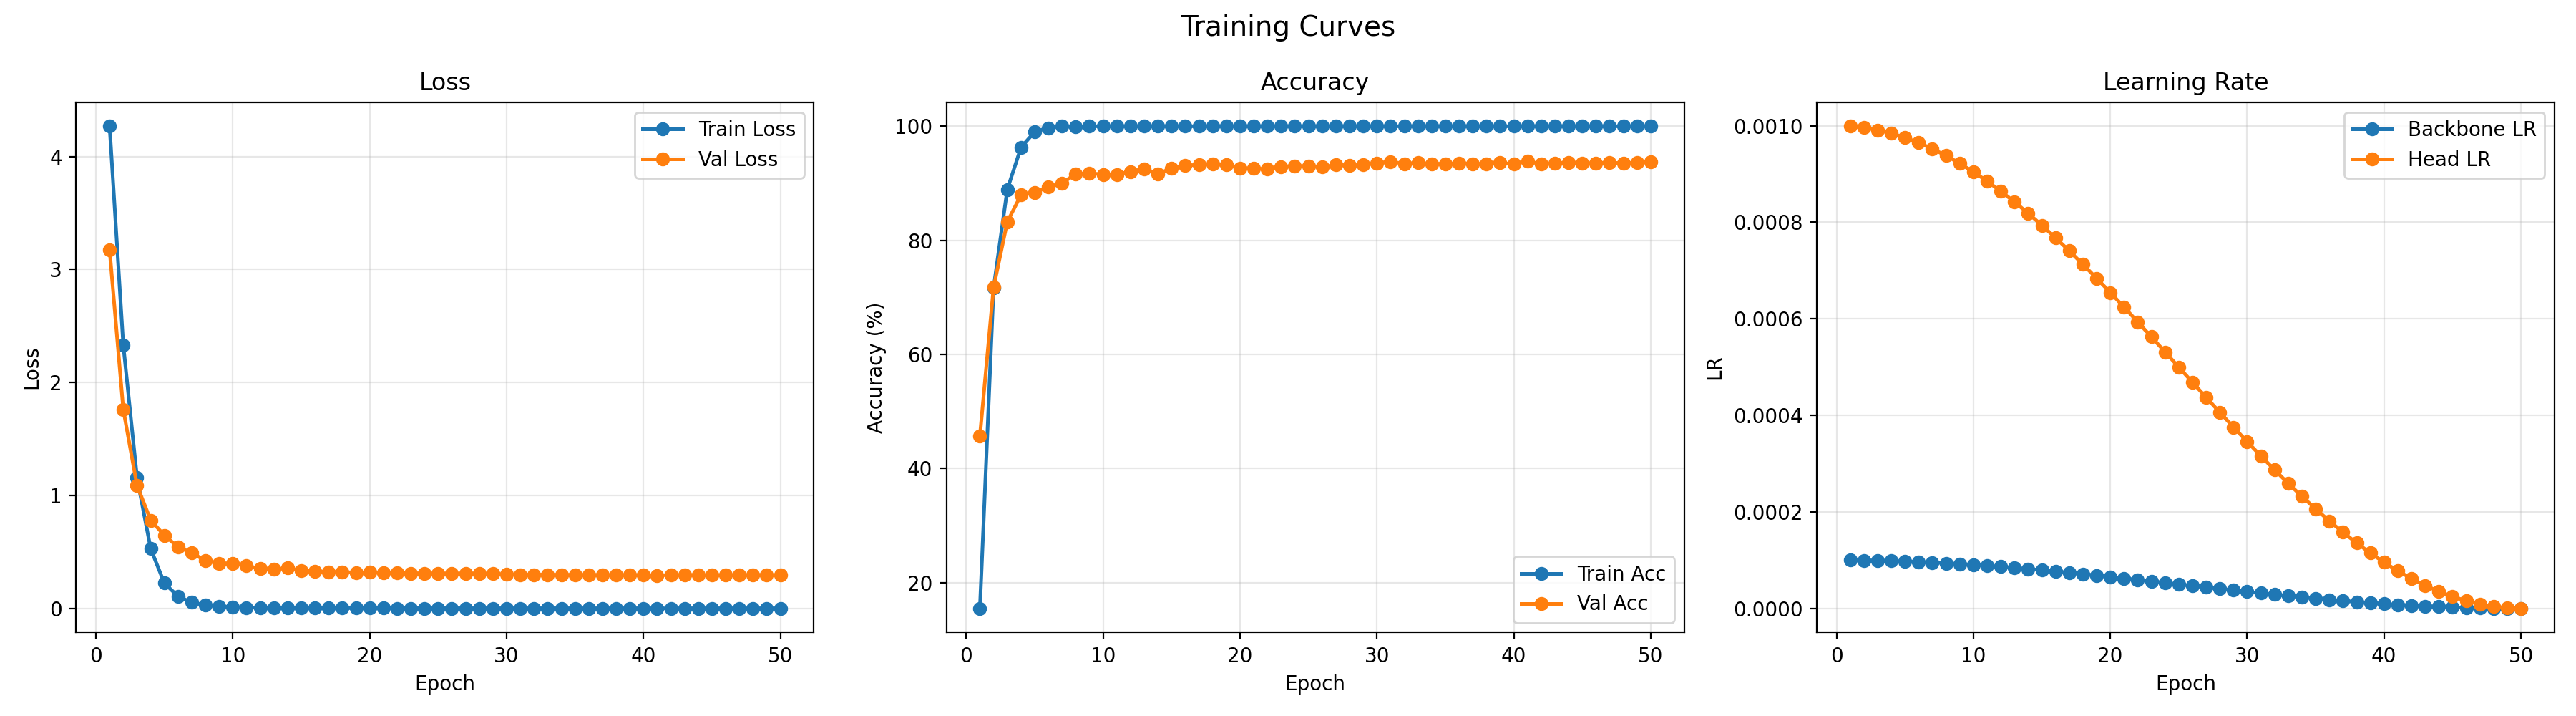
\includegraphics[width=0.95\textwidth]{outputs/figures/hparam_resnet18_lr1_epochs50/training_curves.png}
    \caption{hparam\_resnet18\_lr1\_epochs50 的训练曲线}
    \label{fig:hparam-resnet18-lr1-epochs50-curves}
\end{figure}

\begin{figure}[H]
    \centering
    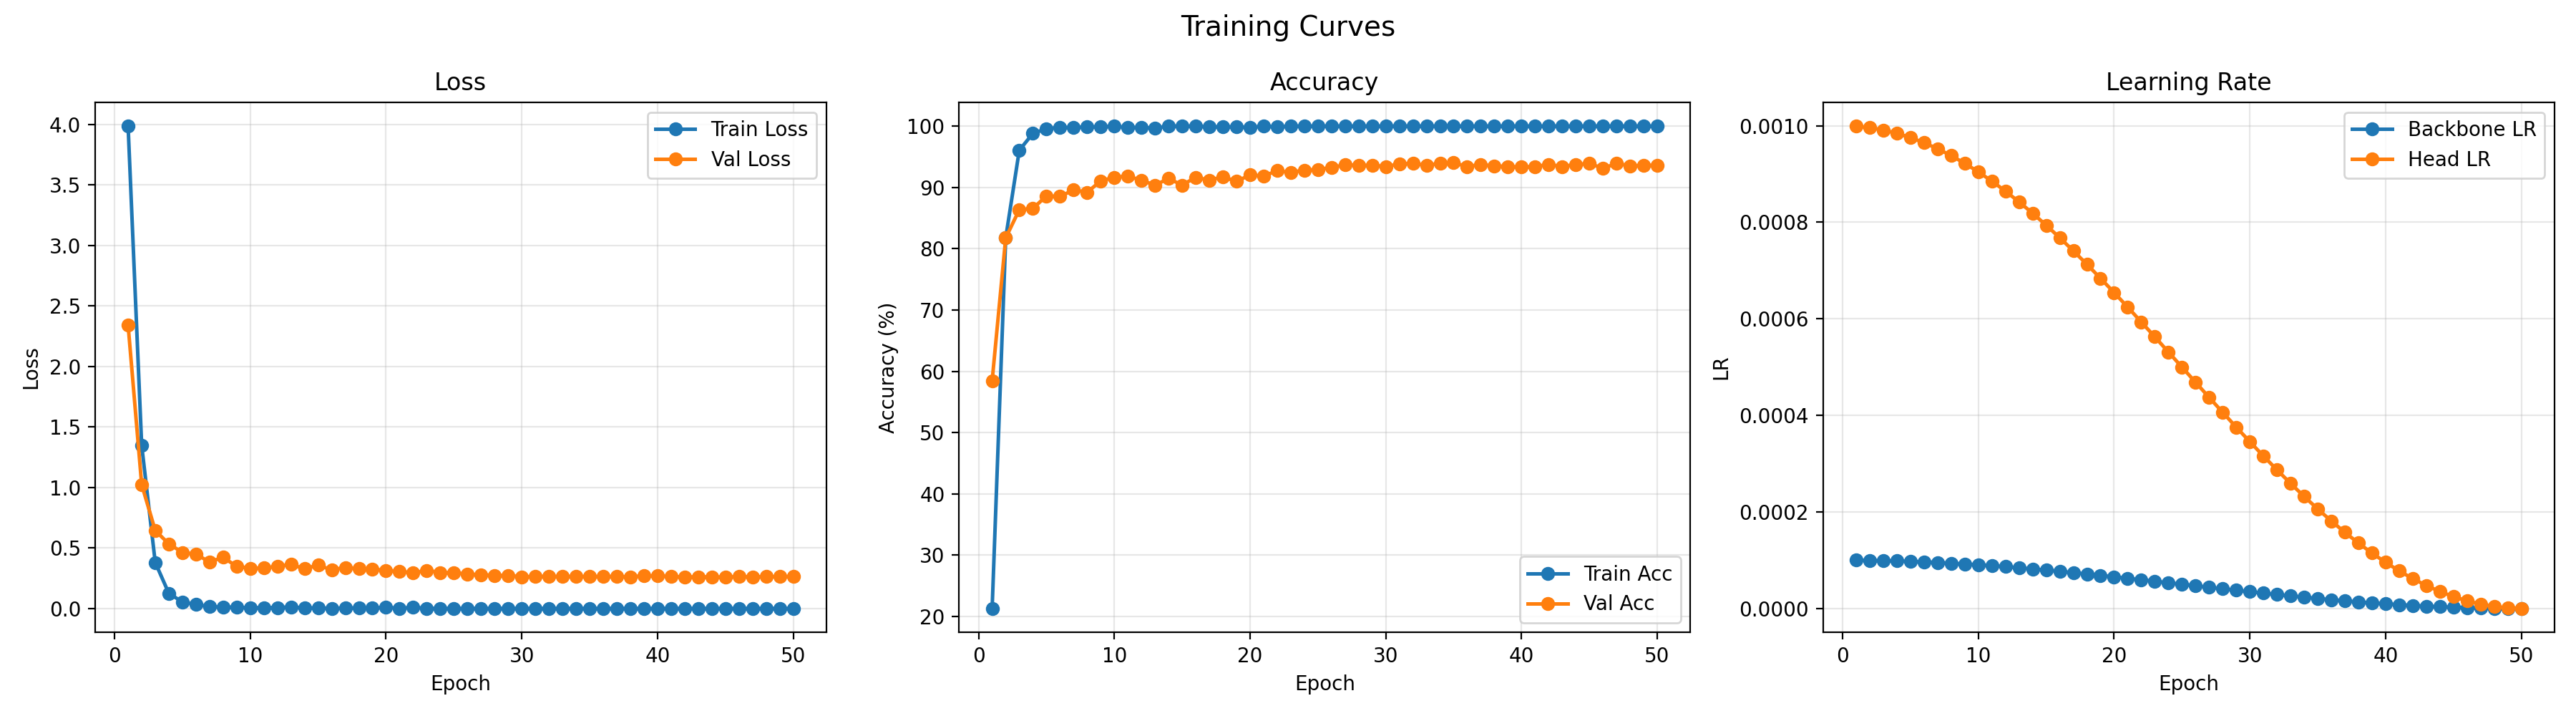
\includegraphics[width=0.95\textwidth]{outputs/figures/hparam_resnet34_lr1_epochs50/training_curves.png}
    \caption{hparam\_resnet34\_lr1\_epochs50 的训练曲线}
    \label{fig:hparam-resnet34-lr1-epochs50-curves}
\end{figure}

\subsection{预训练消融实验}
\begin{table}[H]
\centering
\caption{预训练消融实验结果}
\label{tab:ablation-results}
\resizebox{\textwidth}{!}{
\begin{tabular}{llllrrp{5.2cm}}
\toprule
Backbone & Pretrained & Init Strategy & Best Val Acc(\%) & Test Acc(\%) & Performance Gap(\%) & Analysis \\
\midrule
ResNet-18 & Yes & ImageNet + random head & 93.33 & 90.37 & +53.91 & 预训练模型显著优于随机初始化，说明 ImageNet 特征迁移有效。 \\
ResNet-18 & No & Random initialization & 42.16 & 36.46 & -- & 从零训练难以在有限样本中学习充分通用特征。 \\
ResNet-34 & Yes & ImageNet + random head & 93.92 & 90.40 & +48.46 & 更深模型同样显著受益于 ImageNet 预训练。 \\
ResNet-34 & No & Random initialization & 48.53 & 41.94 & -- & 随机初始化模型测试性能明显不足，泛化能力较弱。 \\
\bottomrule
\end{tabular}}
\end{table}

消融结果表明，ImageNet 预训练对 Flowers102 这种小规模细粒度分类任务具有显著帮助。ResNet-18 pretrained 相比 scratch 测试 Accuracy 提升 53.91 个百分点；ResNet-34 pretrained 相比 scratch 提升 48.46 个百分点。需要说明的是，为了突出初始化方式本身的影响，本实验在 scratch 与 pretrained 对比中保持了相同优化配置。然而，随机初始化网络通常可能需要更大的 backbone 学习率和更长训练轮数，因此 scratch 结果并不代表随机初始化模型在充分调参后的最优性能，而主要用于说明 ImageNet 预训练在相同训练预算下的优势。

为进一步检验上述限制，本文补充了 scratch extended-budget 实验，如表~\ref{tab:extended-scratch-results} 所示。相较 30 epoch 的同预算 scratch，ResNet-18 scratch 在 100 epoch、1e-3 backbone learning rate 下测试 Accuracy 从 36.46\% 提升到 48.87\%；ResNet-34 scratch 从 41.94\% 提升到 49.00\%。这说明随机初始化模型确实受益于更长训练和更大学习率，但即便如此，它们仍显著低于 ImageNet pretrained 模型约 90\% 的测试准确率。因此，扩展实验强化了迁移学习优势的结论，同时也避免将原始 scratch 结果误读为随机初始化模型的充分训练上限。

\begin{table}[H]
\centering
\caption{Scratch extended-budget 实验结果}
\label{tab:extended-scratch-results}
\resizebox{\textwidth}{!}{
\begin{tabular}{llllrrp{5.6cm}}
\toprule
Experiment & Backbone & Epochs & LR 设置 & Best Val Acc(\%) & Test Acc(\%) & Interpretation \\
\midrule
ablation\_resnet18\_scratch & ResNet-18 & 30 & 1e-4 / 1e-3 & 42.16 & 36.46 & 同预算消融结果，用于控制初始化方式。 \\
extended\_scratch\_resnet18\_epochs100\_lr1e3 & ResNet-18 & 100 & 1e-3 / 1e-3 & 54.90 & 48.87 & 长训练显著提升 scratch，但仍远低于 pretrained。 \\
ablation\_resnet34\_scratch & ResNet-34 & 30 & 1e-4 / 1e-3 & 48.53 & 41.94 & ResNet-34 从零训练也明显困难。 \\
extended\_scratch\_resnet34\_epochs100\_lr1e3 & ResNet-34 & 100 & 1e-3 / 1e-3 & 54.51 & 49.00 & 更长训练后提升有限，说明小数据集从零学习强表征仍较困难。 \\
\bottomrule
\end{tabular}}
\end{table}

\subsection{注意力机制实验}
\begin{table}[H]
\centering
\caption{注意力机制对比实验结果}
\label{tab:attention-results}
\resizebox{\textwidth}{!}{
\begin{tabular}{llllrrp{5.2cm}}
\toprule
Method & Backbone & Attention Module & Best Val Acc(\%) & Test Acc(\%) & Params & Observation \\
\midrule
attention\_baseline\_resnet18 & ResNet-18 & None & 93.33 & 90.37 & 11,228,838 & Baseline 表现最好，说明预训练 ResNet-18 已具备较强特征提取能力。 \\
attention\_se\_resnet18 & ResNet-18 & SE, 30 epoch & 92.06 & 89.95 & 11,272,358 & SE 引入通道注意力，但 30 epoch 下未超过 Baseline。 \\
extended\_attention\_se\_resnet18\_epochs50 & ResNet-18 & SE, 50 epoch & 92.55 & 89.97 & 11,272,358 & 延长训练后略有提升，但仍未超过 Baseline。 \\
attention\_cbam\_resnet18 & ResNet-18 & CBAM, 30 epoch & 92.65 & 88.68 & 11,272,750 & CBAM 同时建模通道和空间注意力，但测试集表现低于 Baseline。 \\
extended\_attention\_cbam\_resnet18\_epochs50 & ResNet-18 & CBAM, 50 epoch & 93.04 & 89.35 & 11,272,750 & 延长训练提升验证集表现，但测试集仍未超过 Baseline。 \\
\bottomrule
\end{tabular}}
\end{table}

实验结果显示，SE 和 CBAM 在 30 epoch 主实验以及 50 epoch extended-budget 实验中均未超过普通 ResNet-18 Baseline。这并不意味着注意力机制在所有场景下无效，而说明其效果依赖数据规模、插入位置、优化策略和训练轮数。由于 ResNet 主干来自 ImageNet 预训练，而新增 SE/CBAM 模块是随机初始化的，插入注意力模块会改变原有 stage 输出的特征分布。对于小规模数据集，如果没有采用 identity-like initialization、warm-up 或单独的注意力模块学习率，新增模块不一定能稳定提升泛化能力。扩展实验中 SE 从 89.95\% 提升到 89.97\%，CBAM 从 88.68\% 提升到 89.35\%，说明增加训练轮数可以缓解部分优化不足，但不足以改变 attention 未超过 baseline 的结论。

\subsection{训练曲线与收敛性分析}
训练过程中记录每个 epoch 的 \verb|train_loss|、\verb|val_loss|、\verb|train_acc| 和 \verb|val_acc|，并基于 \verb|metrics.csv| 自动绘制训练曲线。该曲线能够展示训练集与验证集上的 loss 变化，以及验证集 Accuracy 的变化趋势。本实验保存了与在线可视化平台等价的训练过程曲线，曲线由原始训练日志自动生成。由于最终代码提交版本关闭了 wandb/swanlab 在线记录，报告采用本地自动生成的训练曲线作为可视化结果；这些曲线与在线平台曲线使用相同的逐 epoch 标量日志，能够反映训练集和验证集 loss 以及验证集 Accuracy 的变化。

\begin{figure}[H]
    \centering
    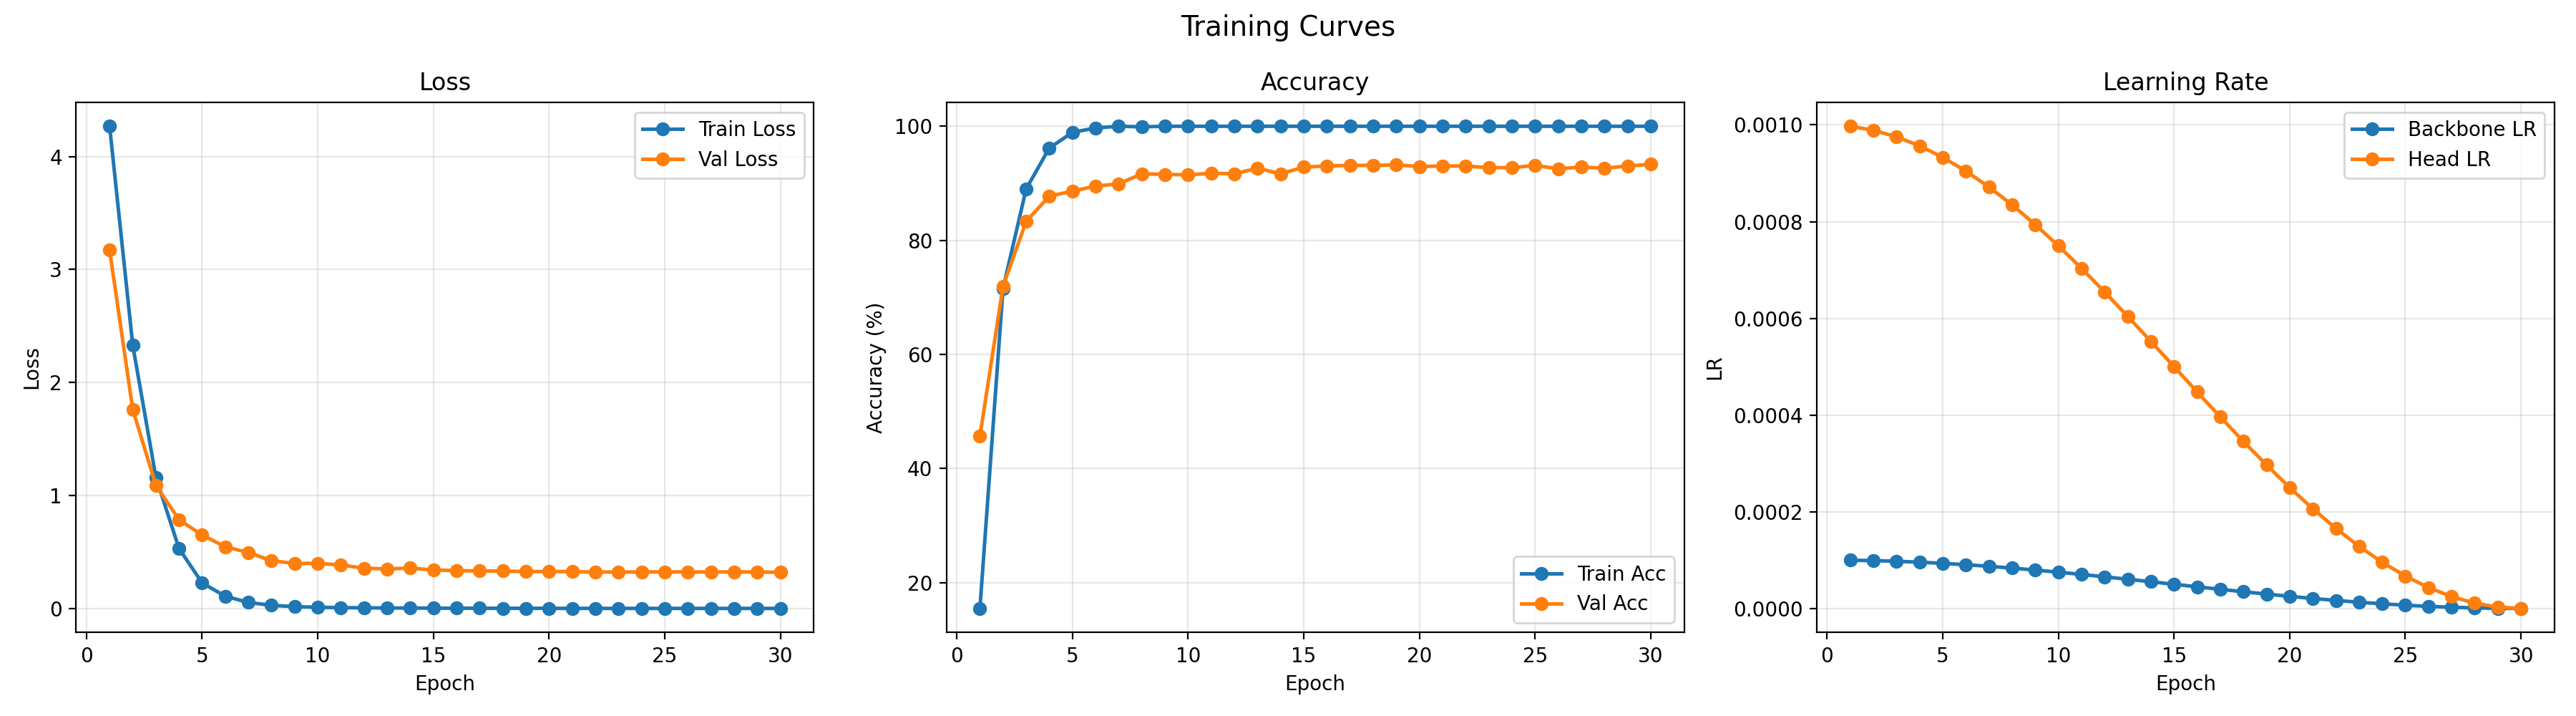
\includegraphics[width=0.95\textwidth]{outputs/figures/baseline_resnet18_pretrained/training_curves.png}
    \caption{baseline\_resnet18\_pretrained 的训练曲线}
    \label{fig:baseline-resnet18-curves}
\end{figure}

\begin{figure}[H]
    \centering
    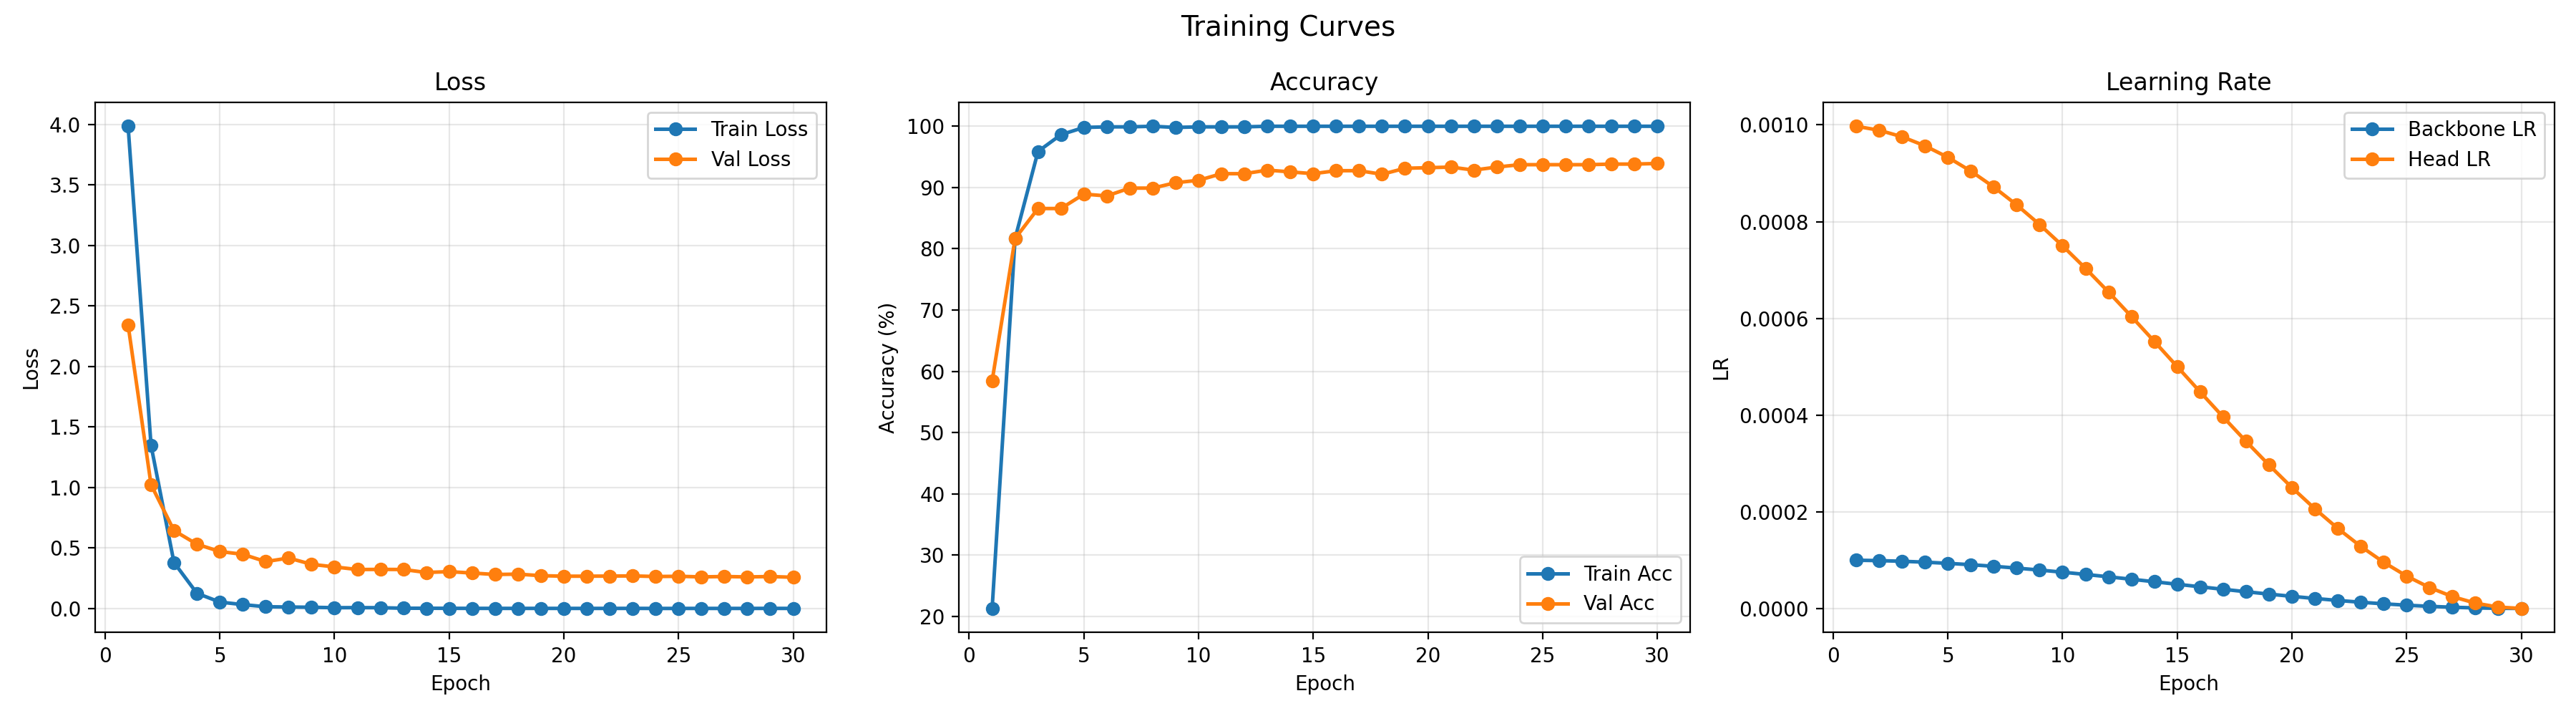
\includegraphics[width=0.95\textwidth]{outputs/figures/baseline_resnet34_pretrained/training_curves.png}
    \caption{baseline\_resnet34\_pretrained 的训练曲线}
    \label{fig:baseline-resnet34-curves}
\end{figure}

\begin{figure}[H]
    \centering
    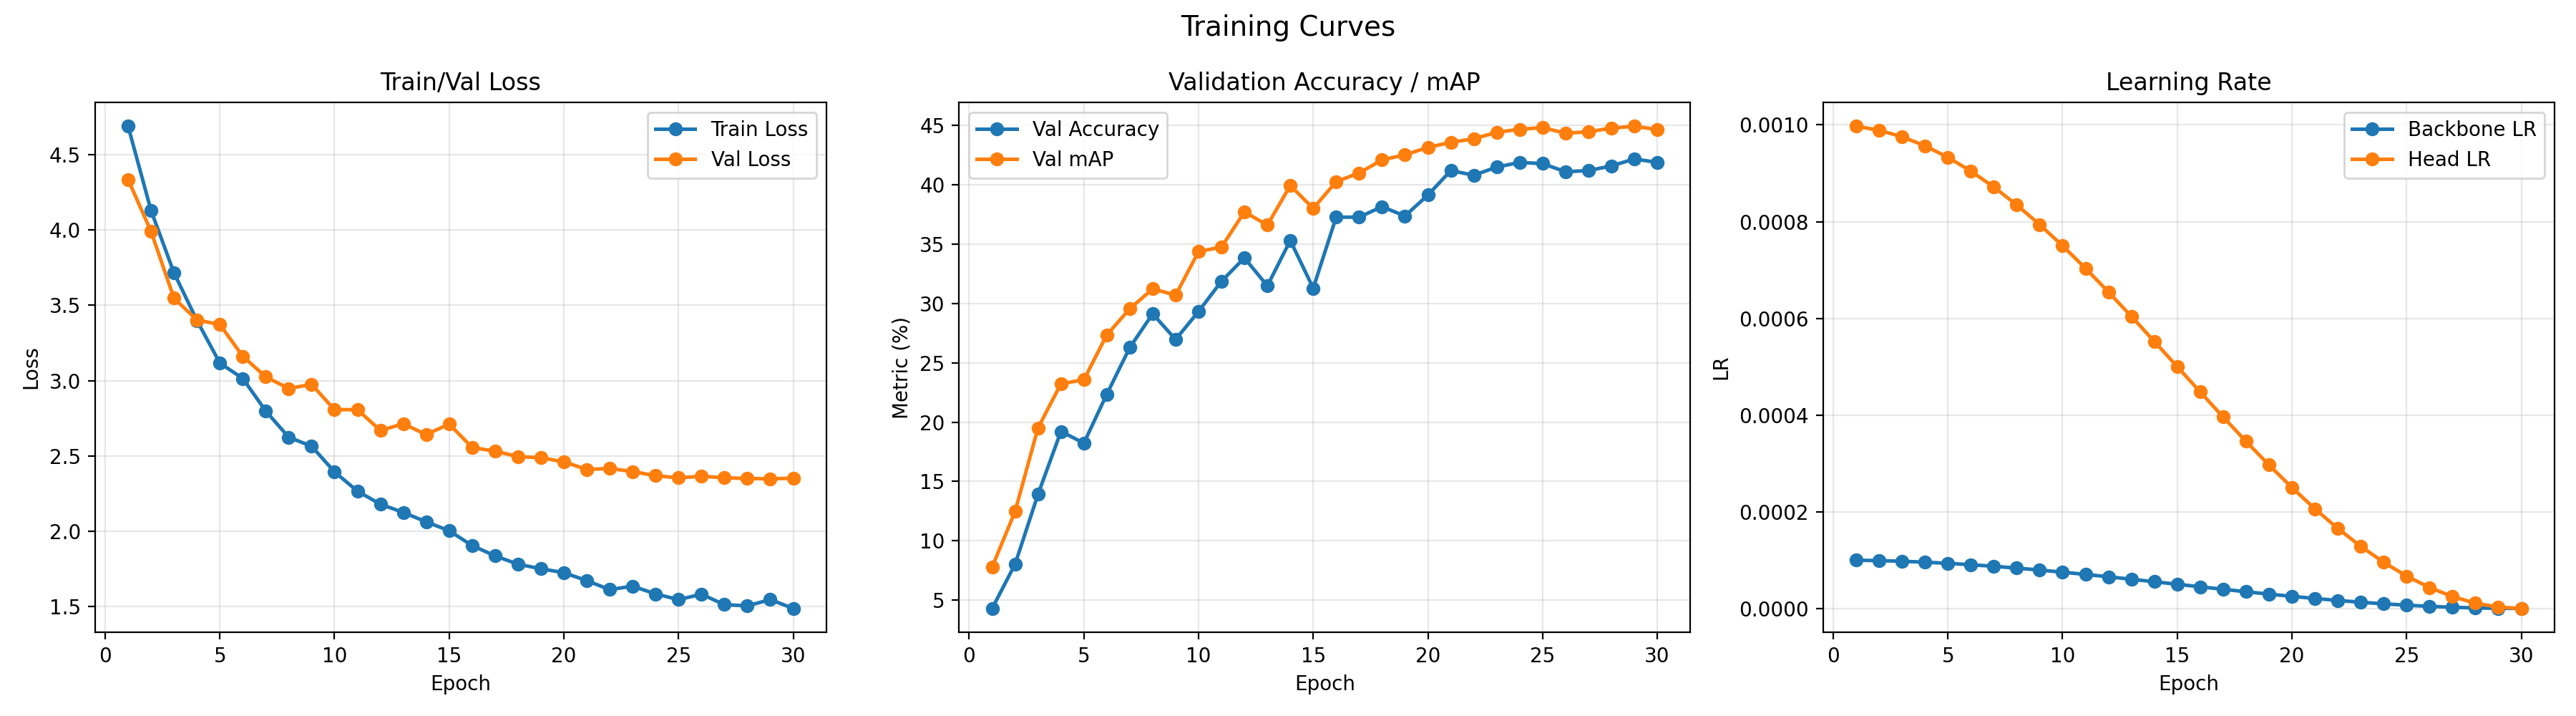
\includegraphics[width=0.95\textwidth]{outputs/figures/ablation_resnet18_scratch/training_curves.png}
    \caption{ablation\_resnet18\_scratch 的训练曲线}
    \label{fig:scratch-resnet18-curves}
\end{figure}

\begin{figure}[H]
    \centering
    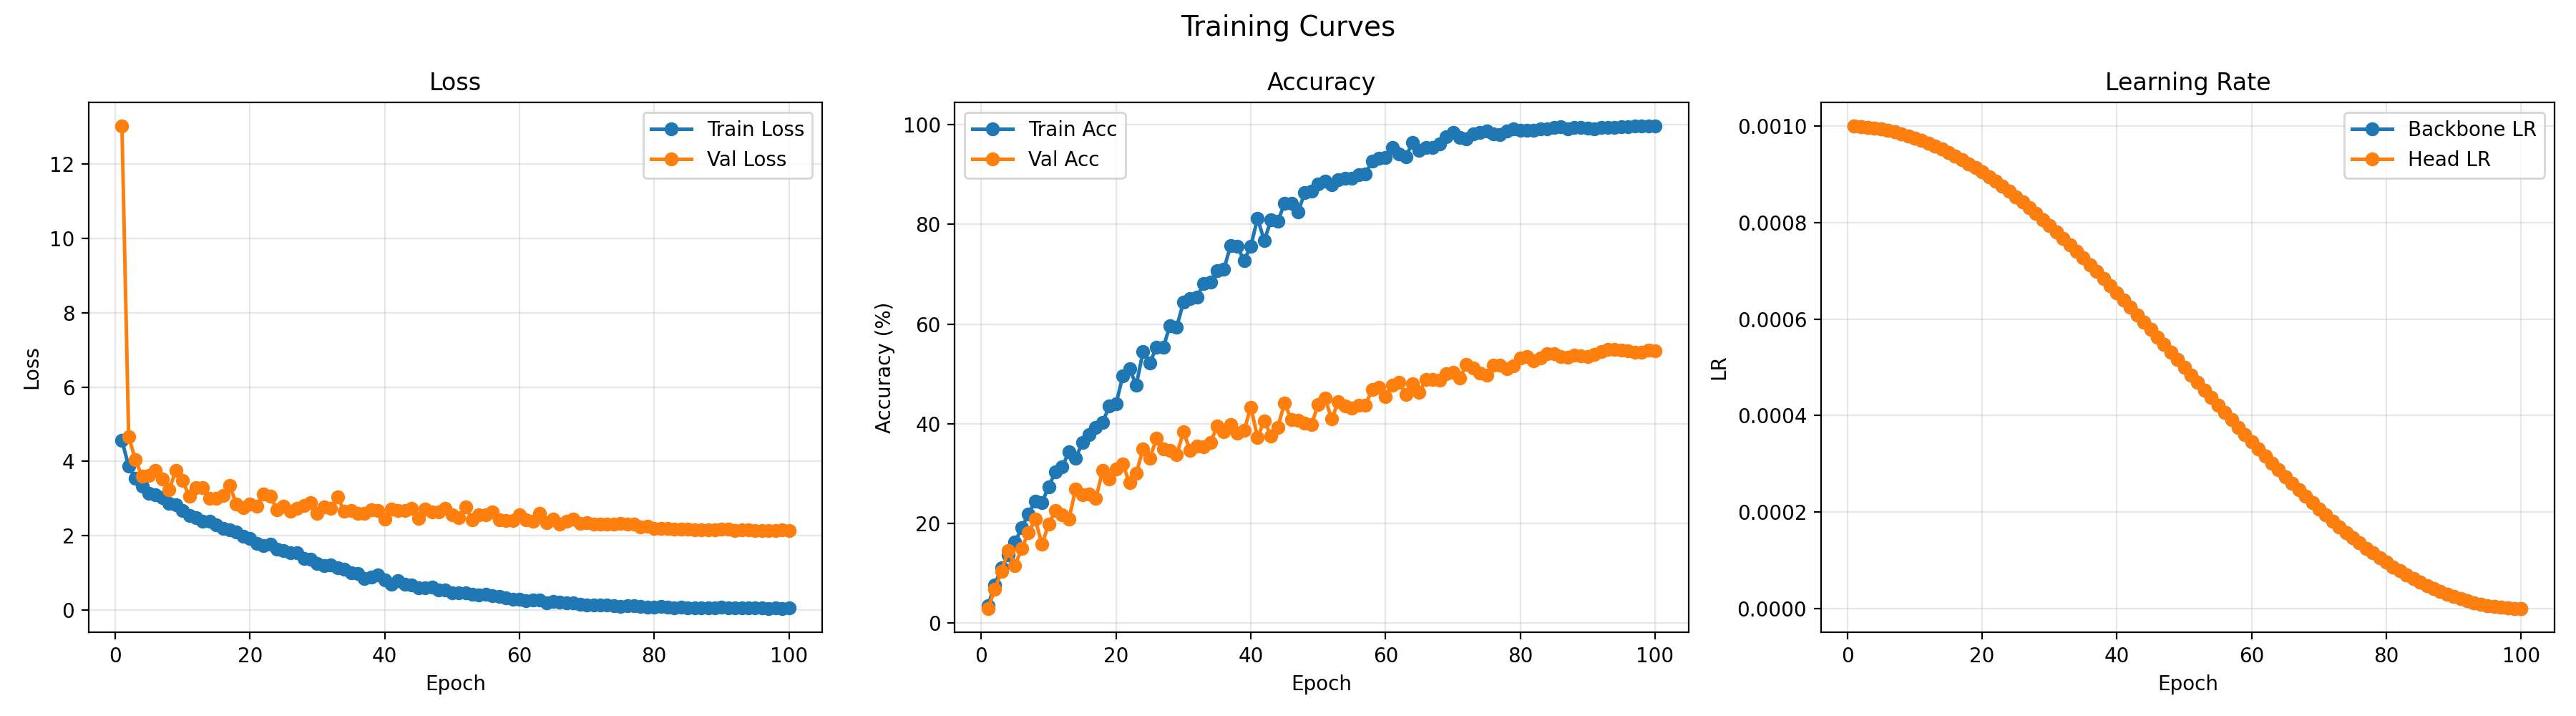
\includegraphics[width=0.95\textwidth]{outputs/figures/extended_scratch_resnet18_epochs100_lr1e3/training_curves.png}
    \caption{extended\_scratch\_resnet18\_epochs100\_lr1e3 的训练曲线}
    \label{fig:extended-scratch-resnet18-curves}
\end{figure}

训练曲线可以分为三类现象理解。第一，pretrained 模型的训练 Accuracy 很快接近 100\%，验证 Accuracy 稳定在 90\% 以上，说明 ImageNet 迁移特征能够快速适配 Flowers102。第二，scratch 模型的 train accuracy 和 val accuracy 均显著低于 pretrained 模型，说明有限训练样本不足以从零学习强表征；extended scratch 的 100 epoch 曲线虽然较 30 epoch scratch 有明显提升，但验证性能仍与 pretrained 存在大幅差距。第三，attention 模型虽然训练集拟合充分，但验证和测试 Accuracy 未超过 baseline，说明新增模块未带来额外泛化收益，甚至可能引入优化难度或轻微过拟合。

\begin{figure}[H]
    \centering
    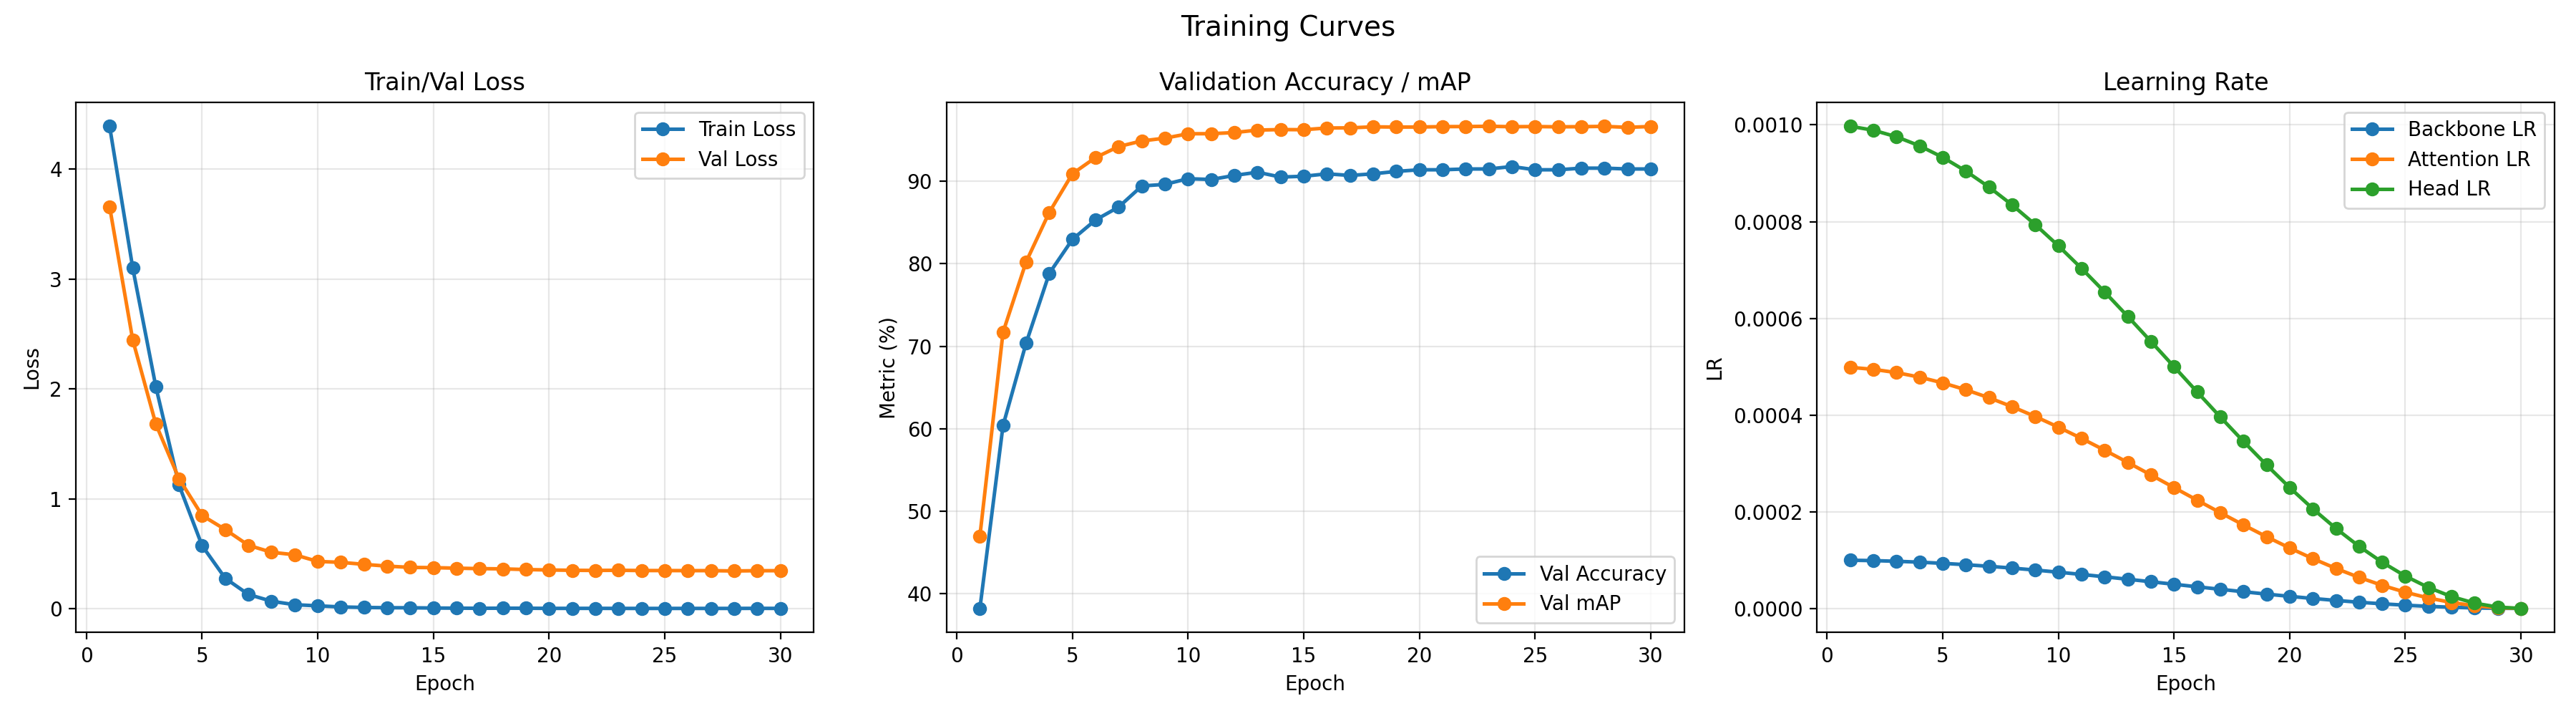
\includegraphics[width=0.95\textwidth]{outputs/figures/attention_se_resnet18/training_curves.png}
    \caption{attention\_se\_resnet18 的训练曲线}
    \label{fig:se-resnet18-curves}
\end{figure}

\begin{figure}[H]
    \centering
    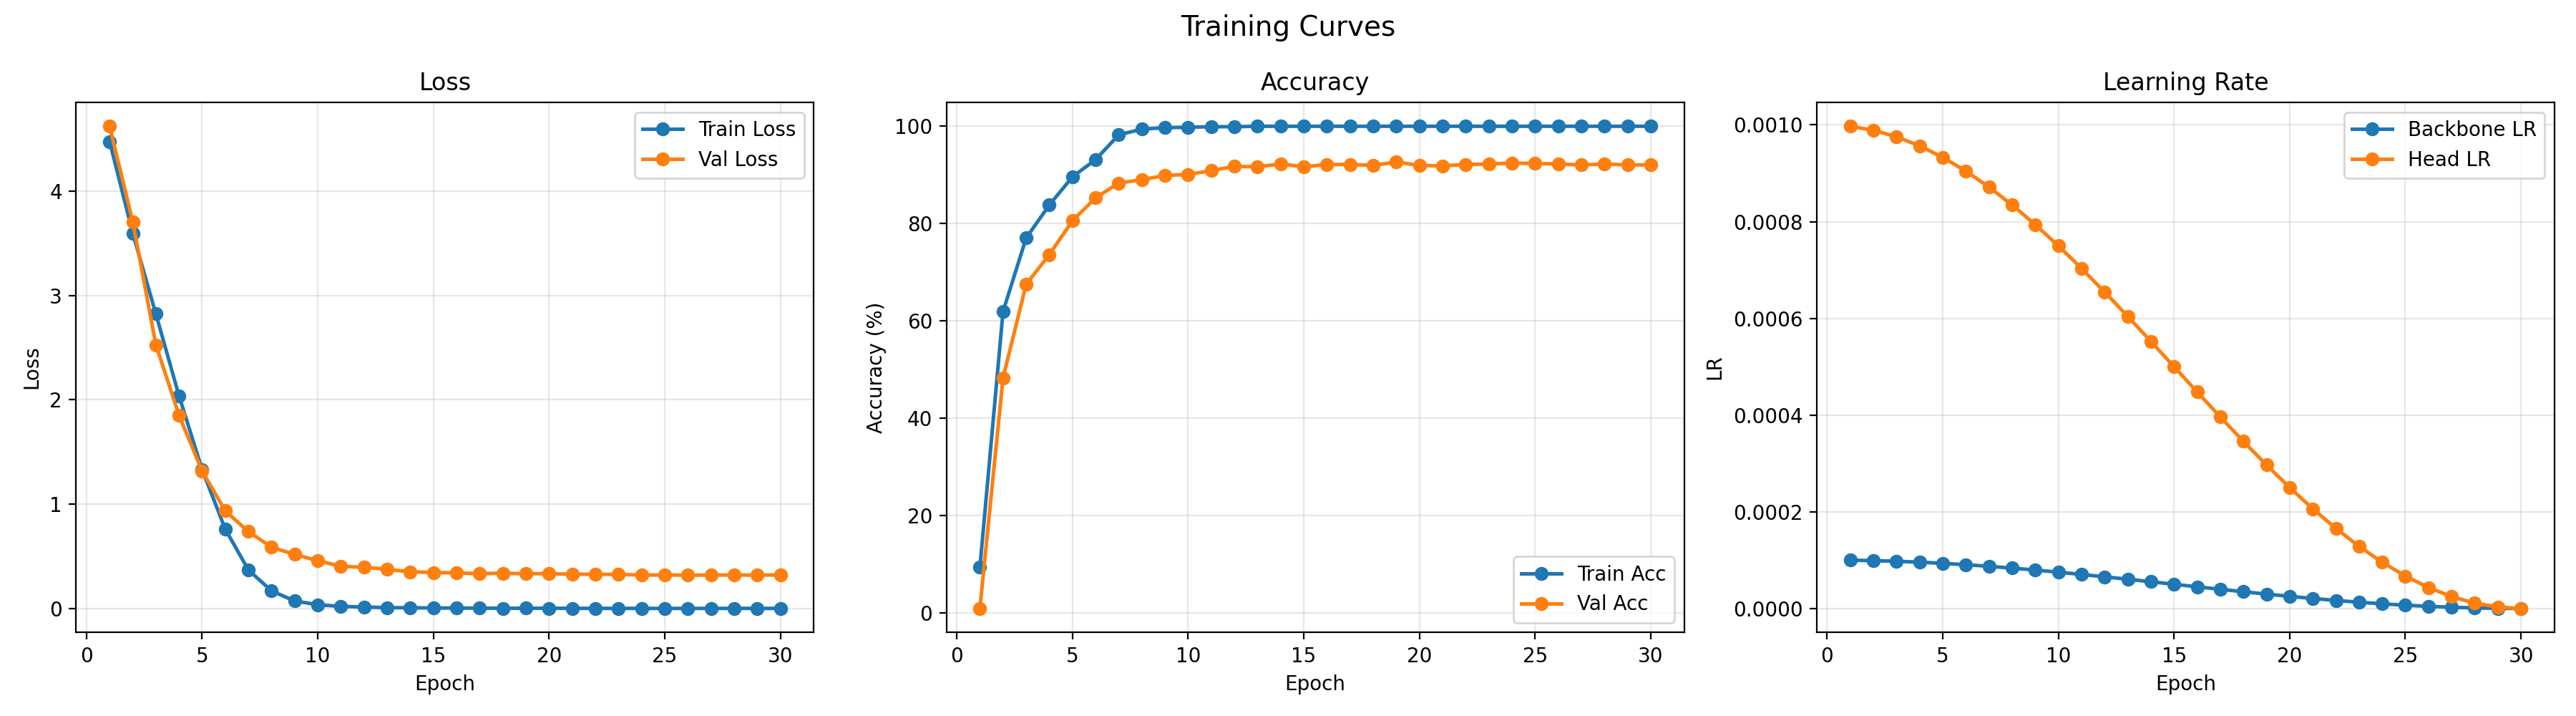
\includegraphics[width=0.95\textwidth]{outputs/figures/attention_cbam_resnet18/training_curves.png}
    \caption{attention\_cbam\_resnet18 的训练曲线}
    \label{fig:cbam-resnet18-curves}
\end{figure}

\begin{figure}[H]
    \centering
    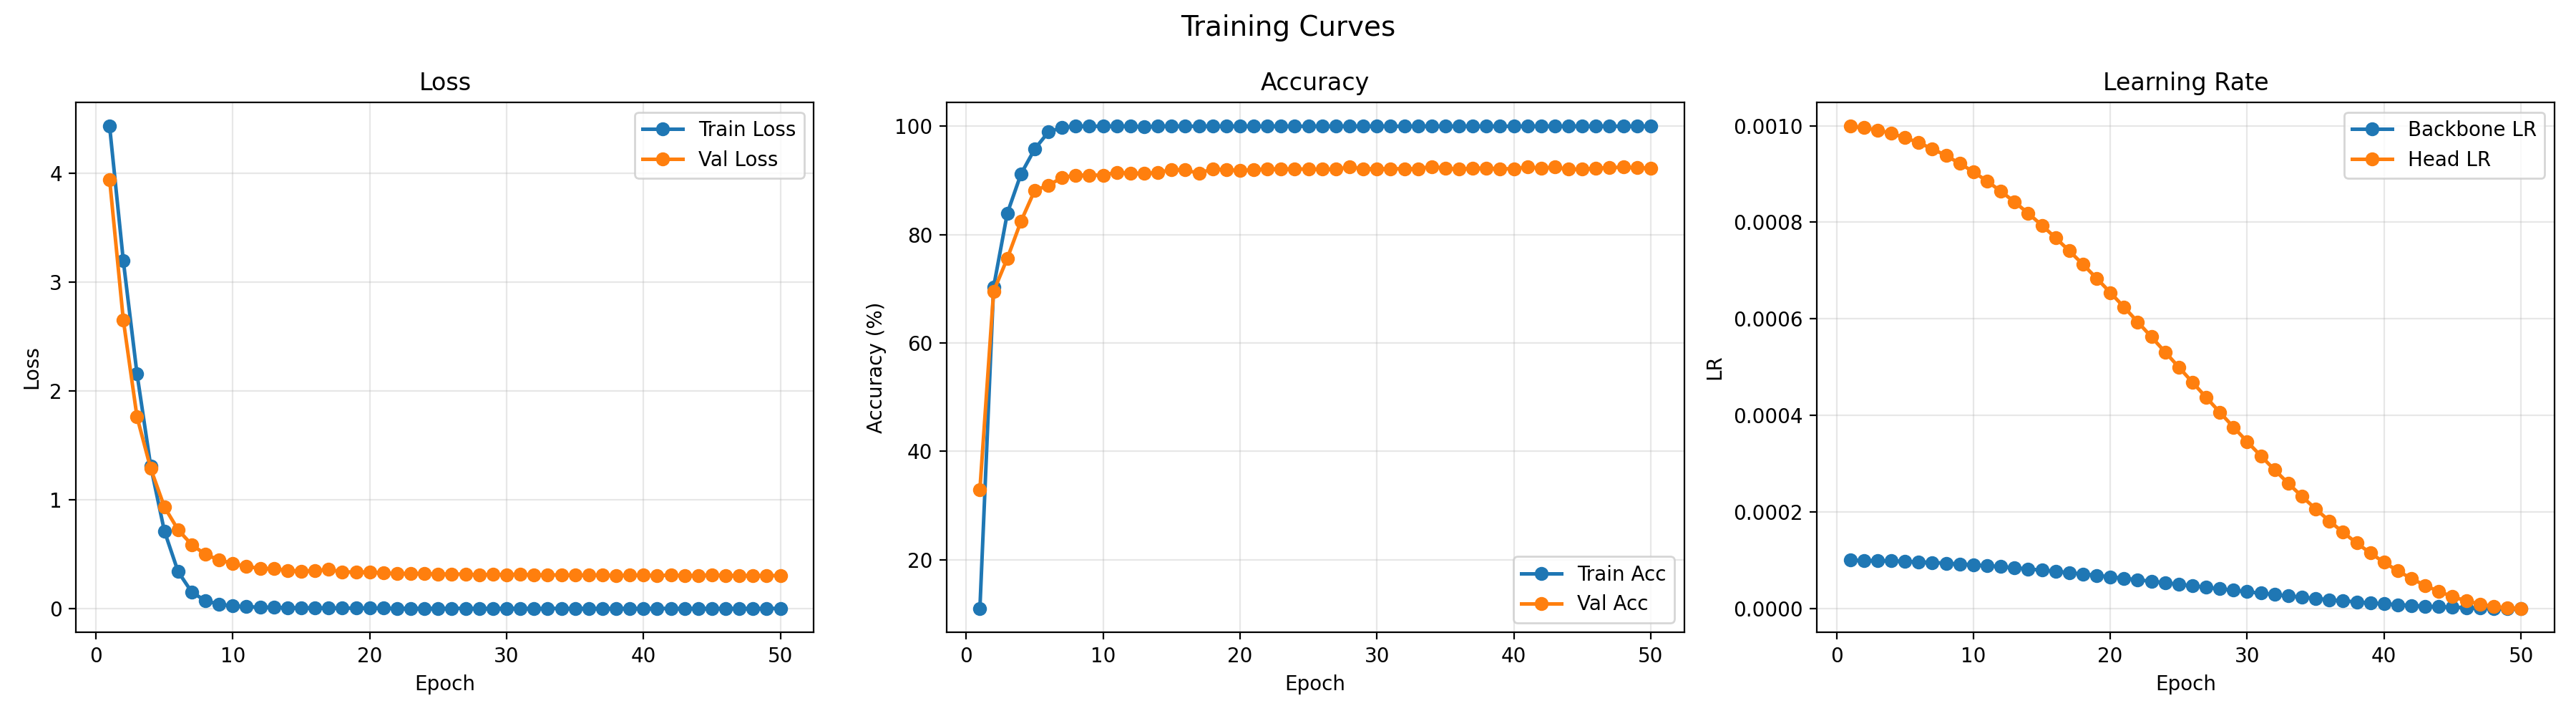
\includegraphics[width=0.95\textwidth]{outputs/figures/extended_attention_se_resnet18_epochs50/training_curves.png}
    \caption{extended\_attention\_se\_resnet18\_epochs50 的训练曲线}
    \label{fig:extended-se-resnet18-curves}
\end{figure}

\begin{figure}[H]
    \centering
    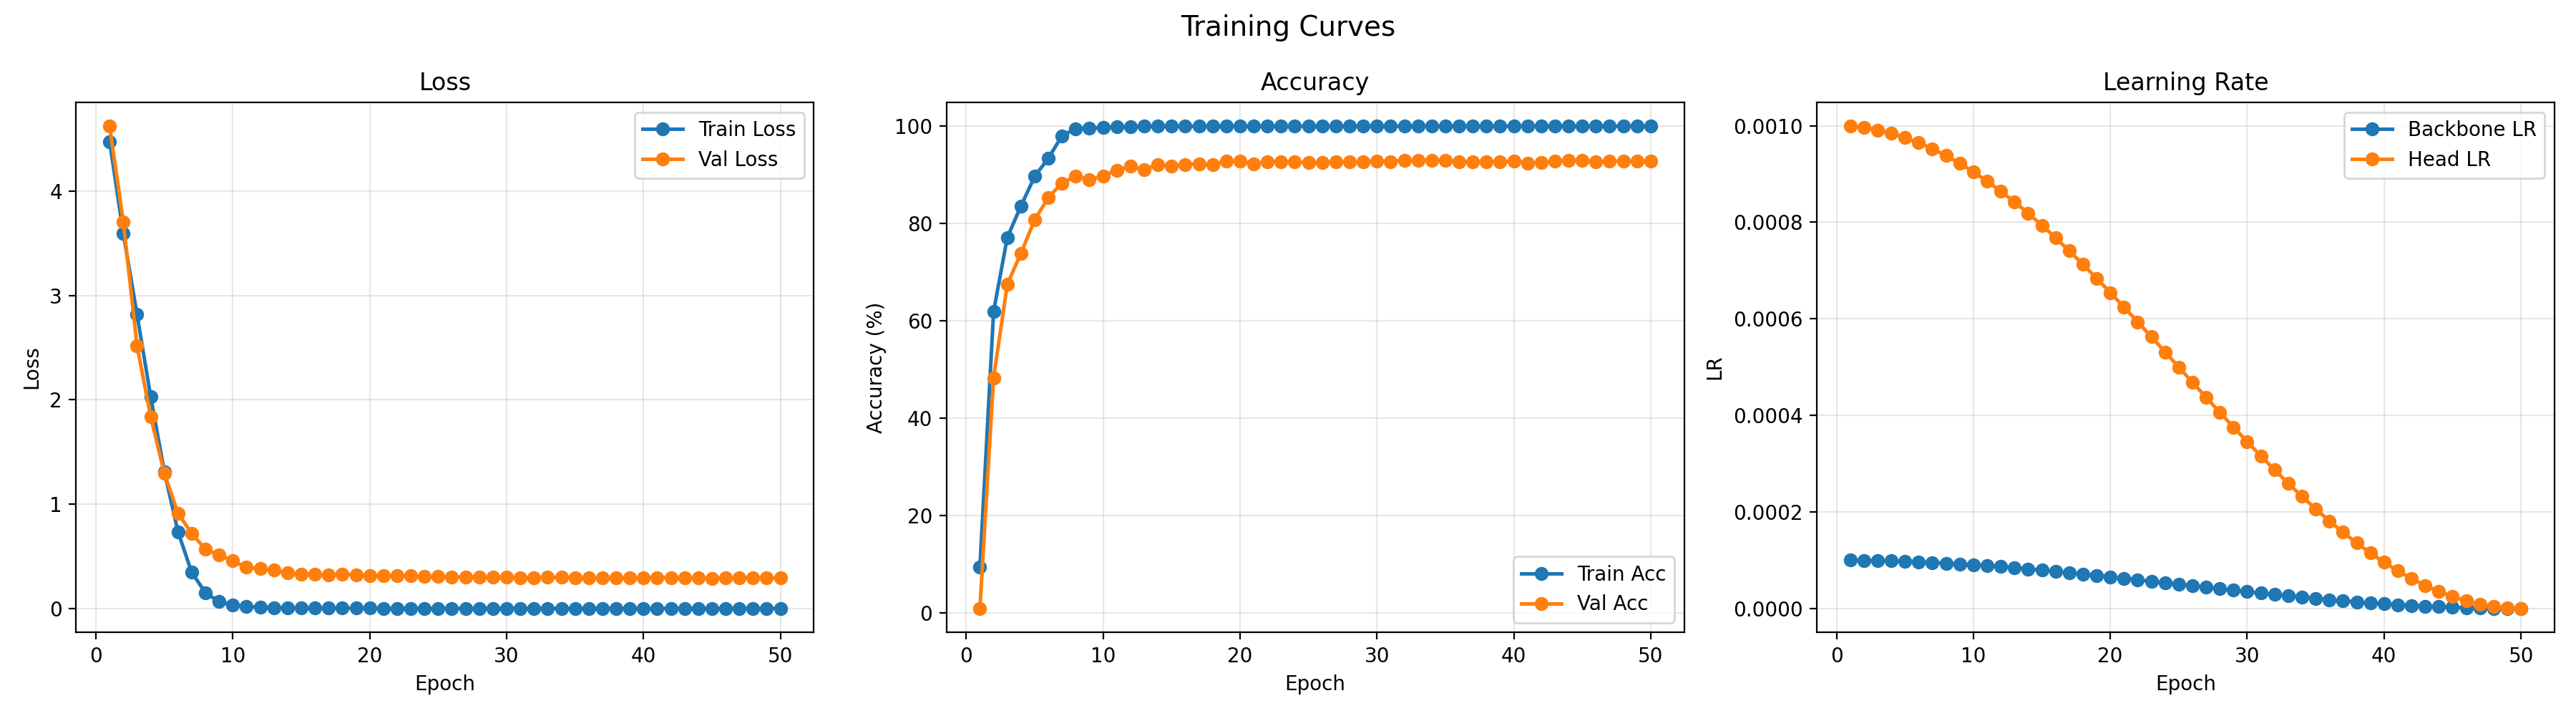
\includegraphics[width=0.95\textwidth]{outputs/figures/extended_attention_cbam_resnet18_epochs50/training_curves.png}
    \caption{extended\_attention\_cbam\_resnet18\_epochs50 的训练曲线}
    \label{fig:extended-cbam-resnet18-curves}
\end{figure}

\subsection{混淆矩阵分析}
混淆矩阵用于观察模型在不同类别上的分类错误分布。Flowers102 类别数量较多，部分类别在颜色、花瓣形状和纹理上较为接近，因此类别间混淆是细粒度图像分类中的常见现象。

\begin{figure}[H]
    \centering
    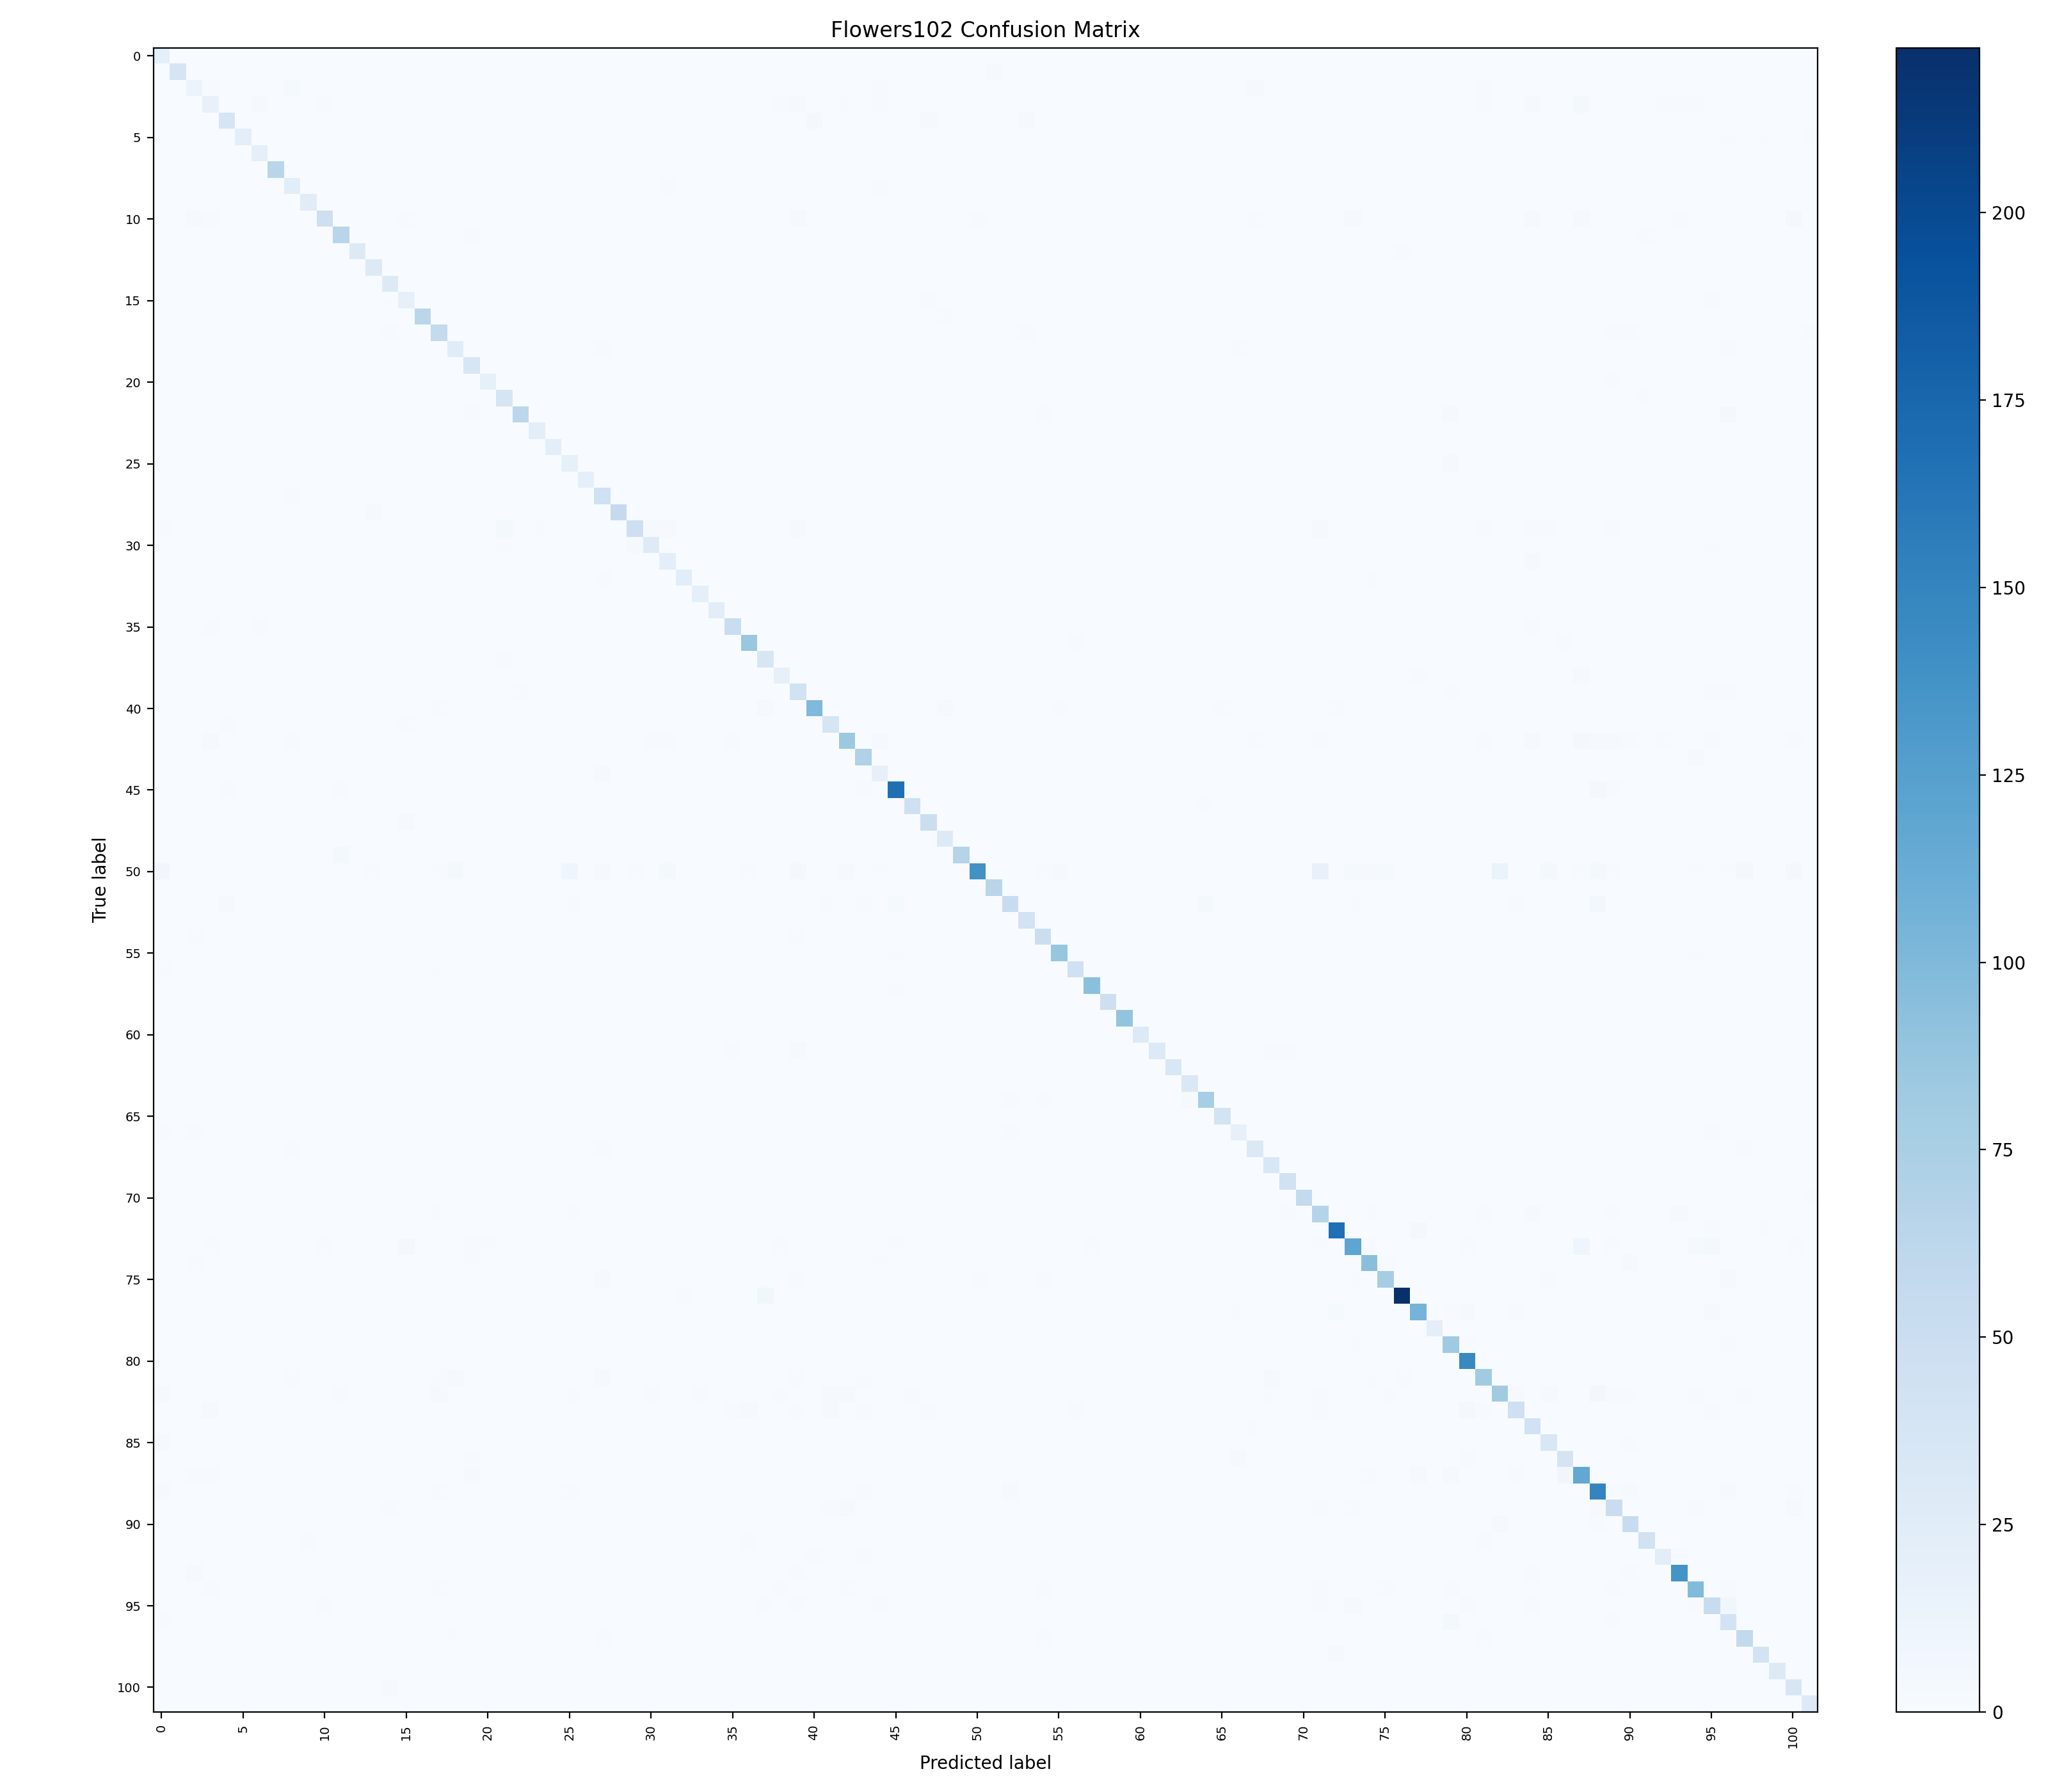
\includegraphics[width=0.95\textwidth]{outputs/figures/baseline_resnet18_pretrained/confusion_matrix.png}
    \caption{baseline\_resnet18\_pretrained 的测试集混淆矩阵}
    \label{fig:baseline-resnet18-confmat}
\end{figure}

\begin{figure}[H]
    \centering
    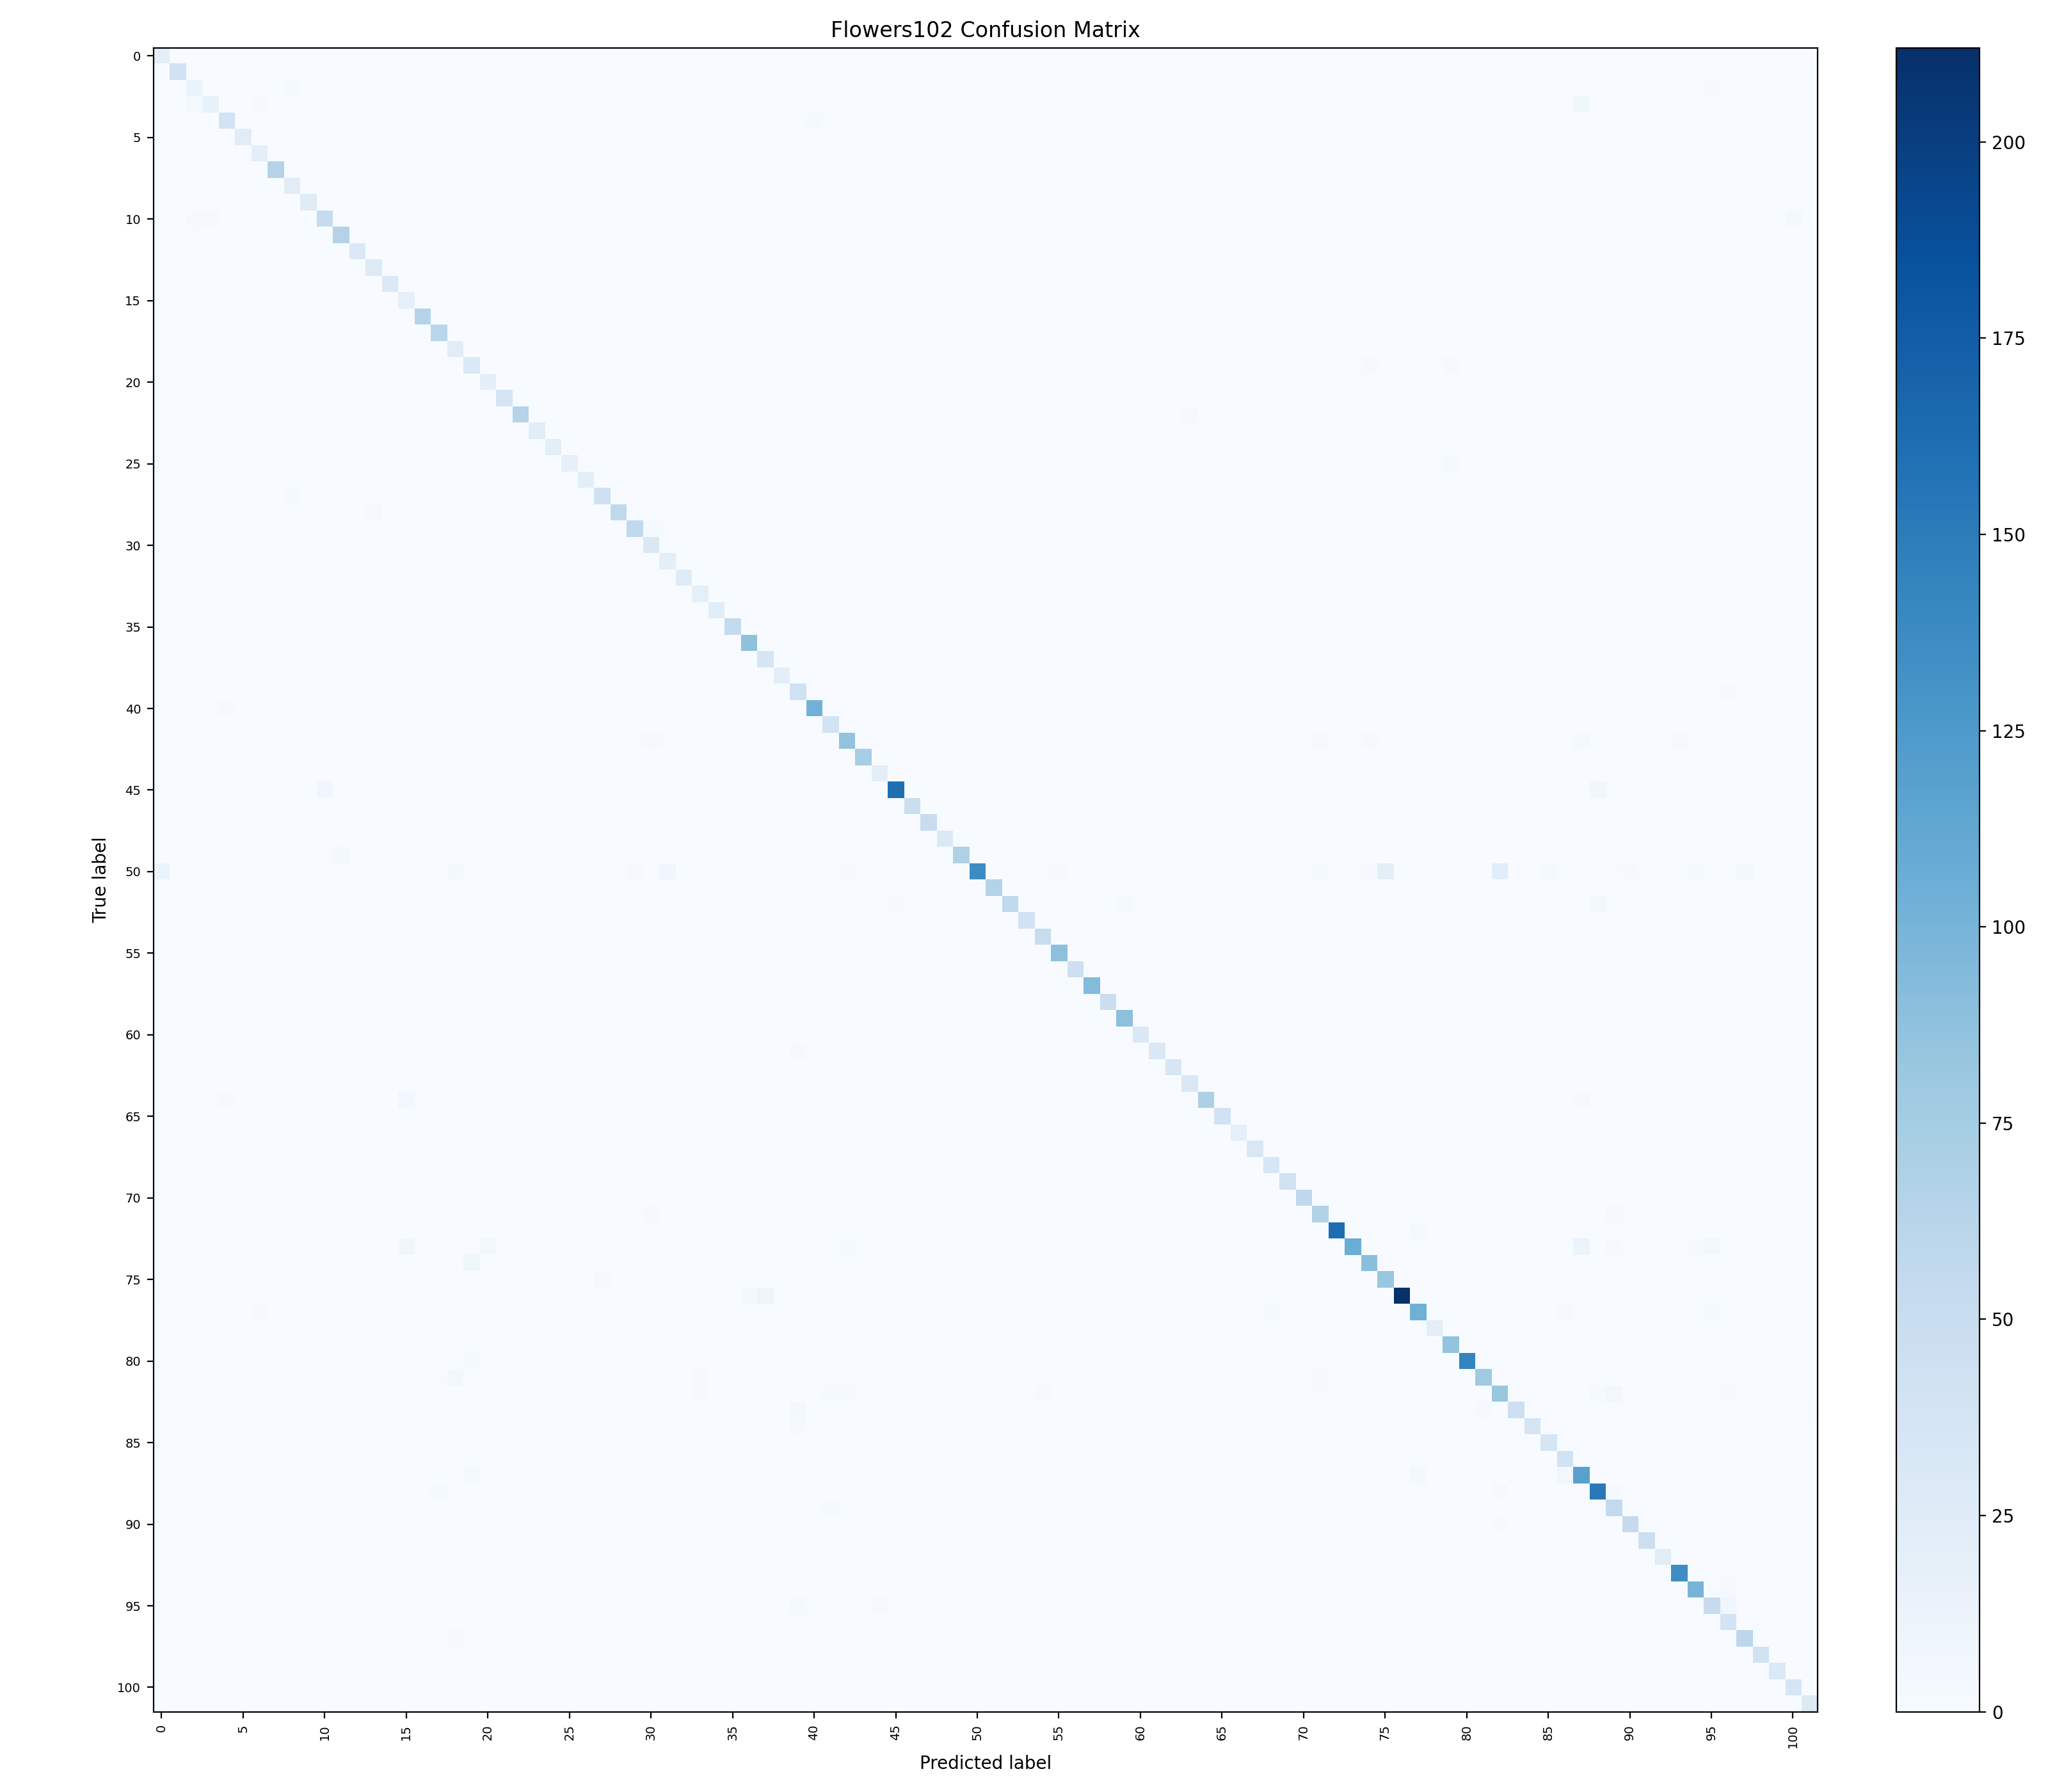
\includegraphics[width=0.95\textwidth]{outputs/figures/baseline_resnet34_pretrained/confusion_matrix.png}
    \caption{baseline\_resnet34\_pretrained 的测试集混淆矩阵}
    \label{fig:baseline-resnet34-confmat}
\end{figure}

\begin{figure}[H]
    \centering
    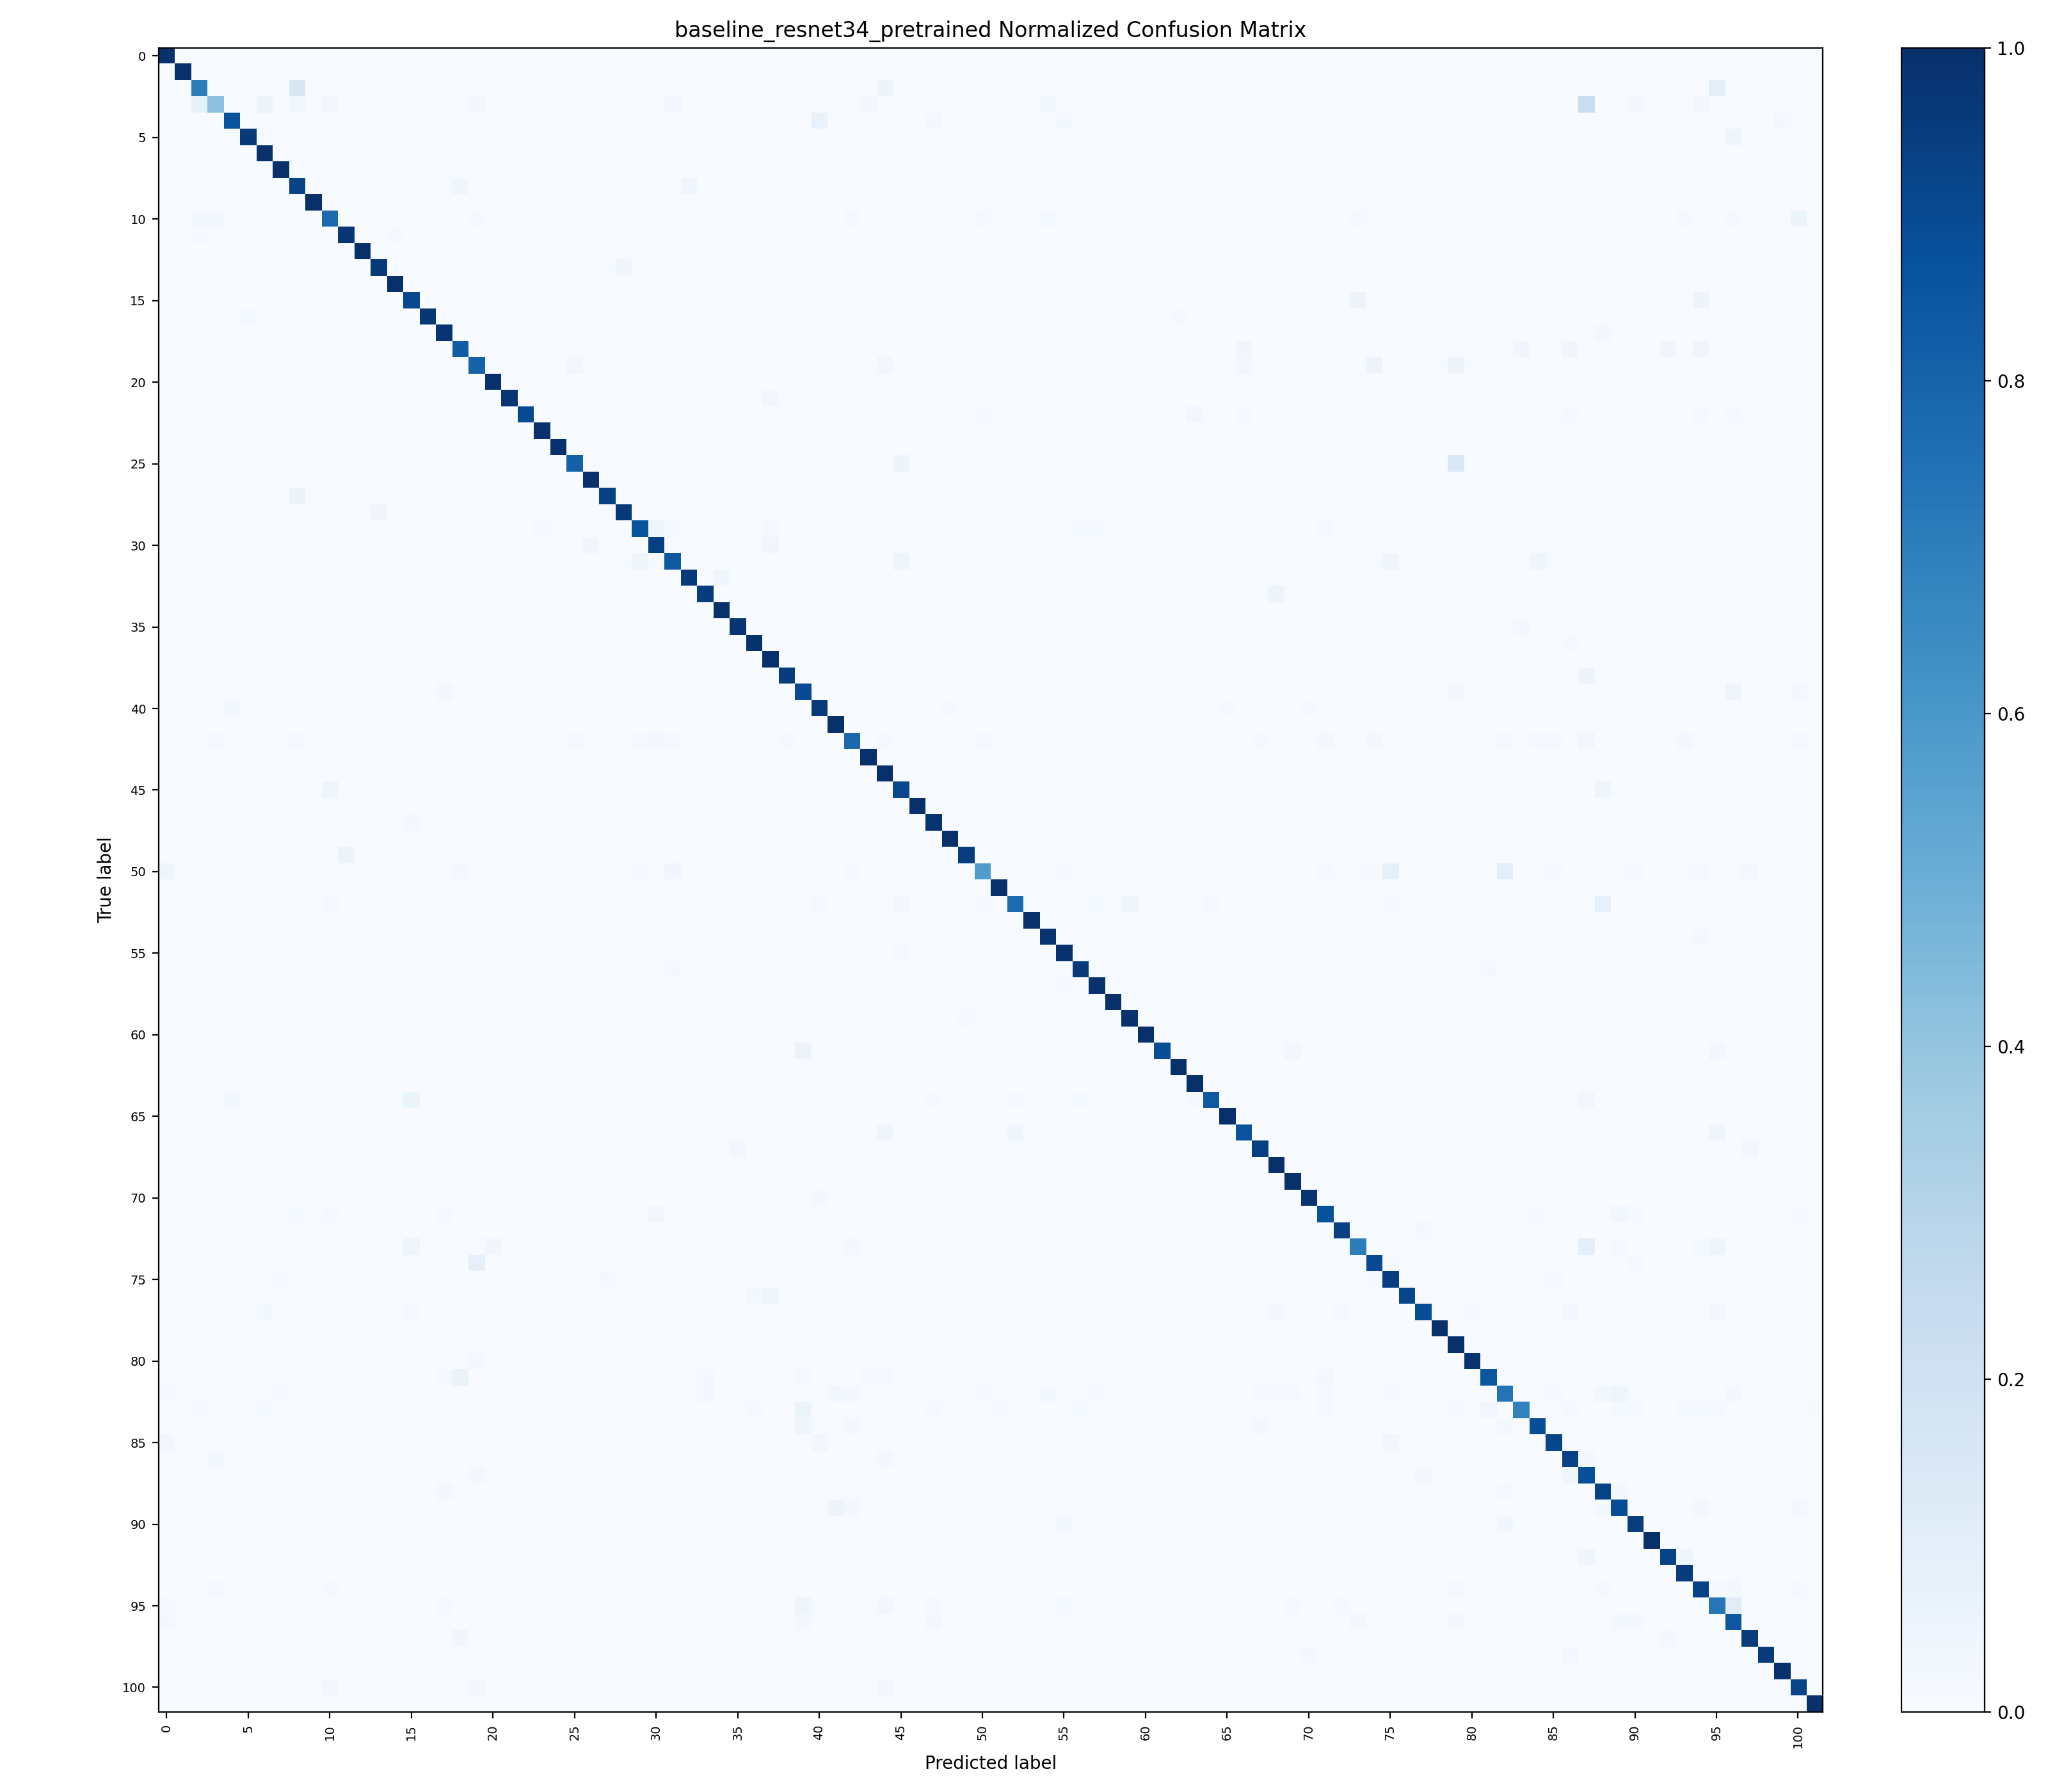
\includegraphics[width=0.95\textwidth]{outputs/figures/baseline_resnet34_pretrained/normalized_confusion_matrix.png}
    \caption{baseline\_resnet34\_pretrained 的归一化测试集混淆矩阵}
    \label{fig:baseline-resnet34-normalized-confmat}
\end{figure}

从混淆矩阵可以分析模型对各类别的区分能力。整体上，预训练 ResNet 能够对大多数类别形成较强判别能力；错误主要集中在视觉外观相似或类内变化较大的花卉类别之间。由于 102 类原始混淆矩阵较密，本文同时给出按真实类别归一化后的混淆矩阵，如图~\ref{fig:baseline-resnet34-normalized-confmat} 所示。归一化形式能够削弱不同类别测试样本数差异的影响，更适合观察单个类别内部的错误比例。

此外，本文使用 \verb|scripts/analyze_confusions.py| 从保存的 \verb|confusion_matrix.npy| 中自动生成 \verb|normalized_confusion_matrix.png|、\verb|top_confusion_pairs.csv| 和 \verb|per_class_accuracy.csv|。这些文件属于结果分析补强产物，不重新训练模型，也不重新评估 checkpoint。基于 baseline\_resnet34\_pretrained 的测试集混淆矩阵，本文提取了非对角线错误数量最高的类别对，如表~\ref{tab:top-confusion-pairs} 所示。类别以 Flowers102 的 class id 表示。

\begin{table}[H]
\centering
\caption{baseline\_resnet34\_pretrained 的 Top-10 混淆类别对}
\label{tab:top-confusion-pairs}
\begin{tabular}{cccp{6.5cm}}
\toprule
True Class ID & Predicted Class ID & Error Count & Possible Reason \\
\midrule
50 & 82 & 23 & 花卉主体颜色或花瓣形态相近，模型易混淆局部纹理。 \\
50 & 75 & 20 & 同一真实类别被分散预测到相似外观类别，说明该类内部变化较大。 \\
73 & 87 & 13 & 类别间形态相似，可能共享相近花瓣轮廓。 \\
50 & 0 & 11 & 类别 50 错误较集中，可能属于难分类或类内差异较大的类别。 \\
76 & 37 & 10 & 视觉结构接近，背景或主体尺度可能影响判别。 \\
95 & 96 & 8 & 相邻 class id 不代表语义相近，但预测结果显示二者视觉特征可能相似。 \\
74 & 19 & 8 & 颜色、纹理或拍摄角度相近导致混淆。 \\
50 & 31 & 8 & 类别 50 再次出现，说明该类别是主要错误来源之一。 \\
45 & 10 & 8 & 可能受花瓣形状和图像背景影响。 \\
3 & 87 & 8 & 类别 3 的 per-class accuracy 较低，模型对该类别泛化不足。 \\
\bottomrule
\end{tabular}
\end{table}

表~\ref{tab:low-per-class} 给出了测试集中 per-class accuracy 最低的若干类别。可以看到，类别 3、50、83、2 和 73 的分类准确率较低，其中类别 50 的测试样本数较多且错误分布明显，说明该类别可能具有较大的类内变化或与多个类别视觉相似。

\begin{table}[H]
\centering
\caption{baseline\_resnet34\_pretrained 中 per-class accuracy 较低的类别}
\label{tab:low-per-class}
\begin{tabular}{ccc}
\toprule
Class ID & Test Samples & Per-class Accuracy(\%) \\
\midrule
3 & 36 & 41.67 \\
50 & 238 & 57.56 \\
83 & 66 & 68.18 \\
2 & 20 & 70.00 \\
73 & 151 & 70.20 \\
95 & 71 & 73.24 \\
82 & 111 & 73.87 \\
52 & 73 & 76.71 \\
10 & 67 & 77.61 \\
42 & 110 & 78.18 \\
\bottomrule
\end{tabular}
\end{table}



\subsection{主要发现总结}

由于部分实验名称对应相同配置，例如 baseline\_resnet18\_pretrained、attention\_baseline\_resnet18、ablation\_resnet18\_pretrained 与 hparam\_resnet18\_lr1\_epochs30 本质上均为 ResNet-18 pretrained baseline，最终不再重复罗列完全相同的行，而是汇总具有代表性的唯一结论，如表~\ref{tab:main-findings} 所示。

\begin{table}[H]
\centering
\caption{主要实验发现总结}
\label{tab:main-findings}
\resizebox{\textwidth}{!}{
\begin{tabular}{p{3.8cm}p{4.2cm}p{3.4cm}p{6.2cm}}
\toprule
Comparison & Representative Result & Key Number & Finding \\
\midrule
Baseline backbone & ResNet-18 vs ResNet-34 pretrained & 90.37\% vs 90.40\% Test Acc & ResNet-34 验证集略高，但测试集仅高 0.03 个百分点，单 seed 下不能认为显著优于 ResNet-18。 \\
Validation-based selection & ResNet-34, 50 epoch, 1e-4/1e-3 & 94.02\% Best Val Acc & 按验证集准则选择时，该设置是最佳模型。 \\
Highest reported test result & ResNet-18 50 epoch lr1; ResNet-34 50 epoch lr2 & 90.57\% Test Acc & 测试集最高观察值不作为超参数选择依据。 \\
Pretraining ablation & ResNet-18 pretrained vs scratch & +53.91 Test Acc points & 相同训练预算下，ImageNet 预训练显著优于随机初始化。 \\
Extended scratch & Scratch 30 epoch vs 100 epoch & 36.46\% to 48.87\%; 41.94\% to 49.00\% & 长训练改善 scratch，但仍远低于 pretrained。 \\
Attention comparison & SE/CBAM 50 epoch vs baseline & 89.97\% / 89.35\% vs 90.37\% & 延长训练后 attention 仍未超过 baseline。 \\
\bottomrule
\end{tabular}}
\end{table}

\section{结论}
本实验完成了基于 ImageNet 预训练 ResNet 的 Flowers102 图像分类任务，并围绕 Baseline、超参数、预训练消融、注意力机制和 extended-budget 设置进行了系统对比。实验结果表明，ImageNet 预训练对 Flowers102 分类任务具有显著帮助。与相同训练预算下的随机初始化相比，ResNet-18 和 ResNet-34 的 pretrained 版本分别在测试 Accuracy 上提升 53.91 和 48.46 个百分点；即使将 scratch 模型扩展到 100 epoch 并提高 backbone learning rate，其测试 Accuracy 仍仅约 49\%，充分说明迁移学习在小规模细粒度图像分类中的有效性。

差分学习率微调策略符合迁移学习场景的训练需求。较小 backbone 学习率有助于保留预训练特征，较大 head 学习率有助于新分类层快速适配 102 类花卉标签空间。超参数实验显示，训练轮数与学习率需要联合分析：ResNet-34 在 50 epoch、1e-4/1e-3 学习率下取得最高验证 Accuracy 94.02\%，是验证集准则下的最佳模型；测试 Accuracy 的最高观察值约为 90.57\%，但该结果仅作为测试集表现汇报，不用于反向选择超参数。

注意力机制实验表明，SE 和 CBAM 在 30 epoch 与 50 epoch 扩展训练下均未超过普通 ResNet-18 Baseline。其原因可能包括新增模块随机初始化、插入模块改变预训练 stage 输出分布、小数据集上额外参数增加优化难度，以及潜在过拟合风险。混淆矩阵后处理进一步给出了 normalized confusion matrix、top confused pairs 和 per-class accuracy，使错误分析不只停留在热力图展示层面。后续工作可从更系统的数据增强、更细粒度学习率搜索、早停机制、更强 backbone、identity-like attention initialization 与更稳定的 attention 插入方式等方向继续改进。


\section{代码与模型权重链接}

本实验代码已提交至 public GitHub 仓库，仓库中包含训练与测试代码、配置文件、实验结果表、训练曲线、混淆矩阵以及报告 \LaTeX{} 源码。根据作业要求，数据集文件、ImageNet 预训练缓存以及训练得到的模型权重不上传至 GitHub。

\begin{itemize}
    \item GitHub 仓库：\url{https://github.com/9902030608jac-dot/flower102_task1}
    \item 模型权重 Google Drive 链接：\url{https://drive.google.com/drive/folders/16jzCBtfwesFbTHLzad11ZXdOw51ncH9-?usp=drive_link}
\end{itemize}

模型权重文件对应项目中的 \verb|outputs/checkpoints/{experiment_name}/best.pt|。下载后可按照仓库中 \verb|MODEL_WEIGHTS.md| 的说明放回对应目录并执行评测。Google Drive 中仅包含训练好的模型权重及其校验说明，不包含 Flowers102 数据集文件。

\section{参考说明}
本实验基于 torchvision 中的 Flowers102 数据集接口完成。ResNet-18 和 ResNet-34 使用 torchvision 提供的 ImageNet 预训练权重。SE 和 CBAM 为在 ResNet stage 后手动加入的注意力模块。实验结果来自项目 \verb|outputs/metrics/| 下保存的 CSV、Markdown 和 JSON 文件。训练曲线、原始混淆矩阵和归一化混淆矩阵来自 \verb|outputs/figures/| 下自动生成或后处理得到的图片文件；top confused pairs 与 per-class accuracy 来自 \verb|scripts/analyze_confusions.py| 对 \verb|confusion_matrix.npy| 的后处理分析。

\begin{thebibliography}{9}
\bibitem{resnet} K. He, X. Zhang, S. Ren, and J. Sun. Deep Residual Learning for Image Recognition. CVPR, 2016.
\bibitem{se} J. Hu, L. Shen, and G. Sun. Squeeze-and-Excitation Networks. CVPR, 2018.
\bibitem{cbam} S. Woo, J. Park, J.-Y. Lee, and I. S. Kweon. CBAM: Convolutional Block Attention Module. ECCV, 2018.
\bibitem{flowers102} M.-E. Nilsback and A. Zisserman. Automated Flower Classification over a Large Number of Classes. ICVGIP, 2008.
\end{thebibliography}

\appendix
\section{附录：项目结构}
\begin{lstlisting}
flower102_task1/
  README.md
  configs/
    baseline_resnet18.yaml
    baseline_resnet34.yaml
    scratch_resnet18.yaml
    se_resnet18.yaml
    sweep_hparams.yaml
  scripts/
    train.py
    eval.py
    summarize_results.py
    run_baseline.sh
    run_ablation.sh
    run_attention.sh
    run_hparam_sweep.sh
    run_extended_budget.sh
    analyze_confusions.py
  src/
    datasets.py
    engine.py
    metrics.py
    logger.py
    transforms.py
    utils.py
    models/
      resnet_baseline.py
      attention.py
      se_resnet.py
      cbam_resnet.py
  outputs/
    checkpoints/
    figures/
    metrics/
\end{lstlisting}

\section{附录：报告插图清单}
\begin{longtable}{p{0.22\textwidth}p{0.70\textwidth}}
\caption{建议插入的训练曲线图路径}
\label{tab:curve-list}\\
\toprule
类型 & 路径 \\
\midrule
\endfirsthead
\toprule
类型 & 路径 \\
\midrule
\endhead
训练曲线 & \verb|outputs/figures/baseline_resnet18_pretrained/training_curves.png| \\
训练曲线 & \verb|outputs/figures/baseline_resnet34_pretrained/training_curves.png| \\
训练曲线 & \verb|outputs/figures/hparam_resnet18_lr1_epochs50/training_curves.png| \\
训练曲线 & \verb|outputs/figures/hparam_resnet34_lr1_epochs50/training_curves.png| \\
训练曲线 & \verb|outputs/figures/ablation_resnet18_pretrained/training_curves.png| \\
训练曲线 & \verb|outputs/figures/ablation_resnet18_scratch/training_curves.png| \\
训练曲线 & \verb|outputs/figures/attention_baseline_resnet18/training_curves.png| \\
训练曲线 & \verb|outputs/figures/attention_se_resnet18/training_curves.png| \\
训练曲线 & \verb|outputs/figures/attention_cbam_resnet18/training_curves.png| \\
训练曲线 & \verb|outputs/figures/extended_scratch_resnet18_epochs100_lr1e3/training_curves.png| \\
训练曲线 & \verb|outputs/figures/extended_attention_se_resnet18_epochs50/training_curves.png| \\
训练曲线 & \verb|outputs/figures/extended_attention_cbam_resnet18_epochs50/training_curves.png| \\
\bottomrule
\end{longtable}

\begin{longtable}{p{0.22\textwidth}p{0.70\textwidth}}
\caption{建议插入的混淆矩阵图路径}
\label{tab:confusion-list}\\
\toprule
类型 & 路径 \\
\midrule
\endfirsthead
\toprule
类型 & 路径 \\
\midrule
\endhead
混淆矩阵 & \verb|outputs/figures/baseline_resnet18_pretrained/confusion_matrix.png| \\
混淆矩阵 & \verb|outputs/figures/baseline_resnet34_pretrained/confusion_matrix.png| \\
混淆矩阵 & \verb|outputs/figures/attention_baseline_resnet18/confusion_matrix.png| \\
混淆矩阵 & \verb|outputs/figures/attention_se_resnet18/confusion_matrix.png| \\
混淆矩阵 & \verb|outputs/figures/attention_cbam_resnet18/confusion_matrix.png| \\
归一化混淆矩阵 & \verb|outputs/figures/baseline_resnet34_pretrained/normalized_confusion_matrix.png| \\
混淆对表 & \verb|outputs/figures/baseline_resnet34_pretrained/top_confusion_pairs.csv| \\
逐类准确率 & \verb|outputs/figures/baseline_resnet34_pretrained/per_class_accuracy.csv| \\
\bottomrule
\end{longtable}

\end{document}
